%─────Lecture 4──────────────────────────────────────────────────────────────────────────────────────────────────────────────────────────────────────
% Chapter "Option Pricing Models" (begun in lec_3) continues here.

% ── Black–Scholes helpers for the Greek pictures in this lecture ──
% Same Abramowitz–Stegun 26.2.17 approximation as lec_3, under fresh names so
% that this file compiles on its own (\lec inputs each file inside a group).
\pgfmathdeclarefunction{gphi}{1}{\pgfmathparse{exp(-0.5*(#1)^2)/sqrt(2*pi)}}
\pgfmathdeclarefunction{gtt}{1}{\pgfmathparse{1/(1+0.2316419*abs(#1))}}
\pgfmathdeclarefunction{gtail}{1}{\pgfmathparse{gphi(#1)*gtt(#1)*(0.319381530+gtt(#1)*(-0.356563782+gtt(#1)*(1.781477937+gtt(#1)*(-1.821255978+gtt(#1)*1.330274429))))}}
\pgfmathdeclarefunction{gcdf}{1}{\pgfmathparse{ifthenelse(#1>0,1-gtail(#1),gtail(#1))}}
% Textbook Figs. 10.1--10.5: X = 50, sigma = 30%, r = 8%; #1 = S, #2 = tau in years.
%   r + sigma^2/2 = 0.125.
\pgfmathdeclarefunction{gx}{2}{\pgfmathparse{(ln((#1)/50)+0.125*(#2))/(0.3*sqrt(#2))}}
\pgfmathdeclarefunction{gdelta}{2}{\pgfmathparse{gcdf(gx(#1,#2))}}
\pgfmathdeclarefunction{gthetac}{2}{\pgfmathparse{-(#1)*gphi(gx(#1,#2))*0.3/(2*sqrt(#2))-0.08*50*exp(-0.08*(#2))*gcdf(gx(#1,#2)-0.3*sqrt(#2))}}
\pgfmathdeclarefunction{gthetap}{2}{\pgfmathparse{-(#1)*gphi(gx(#1,#2))*0.3/(2*sqrt(#2))+0.08*50*exp(-0.08*(#2))*gcdf(-gx(#1,#2)+0.3*sqrt(#2))}}
\pgfmathdeclarefunction{ggamma}{2}{\pgfmathparse{gphi(gx(#1,#2))/((#1)*0.3*sqrt(#2))}}
\pgfmathdeclarefunction{gvega}{2}{\pgfmathparse{(#1)*sqrt(#2)*gphi(gx(#1,#2))}}
\pgfmathdeclarefunction{grhoc}{2}{\pgfmathparse{50*(#2)*exp(-0.08*(#2))*gcdf(gx(#1,#2)-0.3*sqrt(#2))}}
\pgfmathdeclarefunction{grhop}{2}{\pgfmathparse{-50*(#2)*exp(-0.08*(#2))*gcdf(-gx(#1,#2)+0.3*sqrt(#2))}}

%─────§ The binomial option pricing formula──────────────────────────────────────────────────────────────────────────────────────────────────────────
\section{The Binomial Option Pricing Formula}
\label{sec:bopm-formula}
\marginpar{\footnotesize\textsf{\raggedright Lecture 4\\ October 1, 2026}}

\source{Slides p.~275}

\autoref{sec:self-financing} showed that the tree is a hedging recipe.
This lecture turns it into a \emph{formula} and then into \emph{algorithms}, takes its limit to reach the Black--Scholes formula, and finally asks how sensitive the answer is to each of its inputs.

The weights in \eqref{eq:bopm-call-n} are binomial probabilities, so name them.

\begin{definition}
	Denote the \vocab{binomial distribution} with parameters $n$ and $p$ by
	\[
		b(j;n,p) \;\triangleq\; \binom{n}{j}p^{j}(1-p)^{n-j} \;=\; \frac{n!}{j!\,(n-j)!}\,p^{j}(1-p)^{n-j} ,
	\]
	where $n!=1\times2\times\cdots\times n$ and, by convention, $0!=1$.
\end{definition}

If you flip a coin $n$ times with $p$ being the probability of getting heads, then $b(j;n,p)$ is the probability of getting $j$ heads.
In the tree, a ``head'' is an up move and $p$ is the risk-neutral probability \eqref{eq:risk-neutral-p}.

\source{Slides pp.~276--277}

The stock prices at time $n$ are $Su^{n},Su^{n-1}d,\ldots,Sd^{n}$, increasing in the number $j$ of up moves.
So the call finishes in the money exactly when $j$ is large enough.

\begin{definition}
	Let $a$ be the minimum number of upward price moves for the call to finish in the money, i.e., the smallest nonnegative integer $j$ such that $Su^{j}d^{n-j}\ge X$.
	Taking logarithms, $j\ln(u/d)\ge\ln\bigl(X/(Sd^{n})\bigr)$, so
	\begin{equation}
		a \;=\; \max\left(0,\ \left\lceil\frac{\ln\bigl(X/(Sd^{n})\bigr)}{\ln(u/d)}\right\rceil\right) .
		\label{eq:bopm-a}
	\end{equation}
\end{definition}

Every term of \eqref{eq:bopm-call-n} with $j<a$ is zero, and for $j\ge a$ the $\max$ can be dropped.
Hence
\begin{align}
	C & \;=\; \frac{\sum_{j=a}^{n}\binom{n}{j}p^{j}(1-p)^{n-j}\bigl(Su^{j}d^{n-j}-X\bigr)}{R^{n}}
	\label{eq:bopm-call-a} \\
	  & \;=\; S\sum_{j=a}^{n}\binom{n}{j}\frac{(pu)^{j}\bigl[(1-p)\,d\bigr]^{n-j}}{R^{n}}
	\;-\; \frac{X}{R^{n}}\sum_{j=a}^{n}\binom{n}{j}p^{j}(1-p)^{n-j}
	\notag \\
	  & \;=\; S\sum_{j=a}^{n}b\bigl(j;n,pu/R\bigr) \;-\; Xe^{-\hat{r}n}\sum_{j=a}^{n}b(j;n,p) .
	\label{eq:bopm-formula}
\end{align}

\begin{note}
	第二行只是把 $S$ 提出來，並把 $R^{n}$ 平均分給每一期：
	\[
		p^{j}(1-p)^{n-j}\cdot\frac{Su^{j}d^{n-j}}{R^{n}} \;=\; S\Bigl(\frac{pu}{R}\Bigr)^{j}\Bigl(\frac{(1-p)\,d}{R}\Bigr)^{n-j} .
	\]
	第三行要把這寫成 $b(j;n,pu/R)$，前提是「上漲」機率 $pu/R$ 和「下跌」機率 $(1-p)d/R$ 加起來剛好是 $1$，而這正是 \eqref{eq:rn-stock} 兩邊同除以 $RS$：
	\[
		\frac{pu}{R}+\frac{(1-p)\,d}{R} \;=\; \frac{pu+(1-p)\,d}{R} \;=\; 1 .
	\]
	（另外 $X/R^{n}=Xe^{-\hat{r}n}$ 是因為 $R=e^{\hat{r}}$。）
	所以 \eqref{eq:bopm-formula} 可以讀成
	\[
		C \;=\; S\times\Pr\nolimits_{pu/R}[\,j\ge a\,] \;-\; \mathrm{PV}(X)\times\Pr\nolimits_{p}[\,j\ge a\,] ,
	\]
	兩項都是「至少上漲 $a$ 次」（即到期 in the money）的機率，差別只在擲哪一枚硬幣：第二項用 risk-neutral probability $p$，第一項用 $pu/R$，它把上漲的權重乘上 $u/R>1$，比 $p$ 更偏向上漲。
	\autoref{thm:black-scholes} 也是完全相同的形狀。
\end{note}

\begin{remark}
	\vocab{二項式選擇權定價公式}（binomial option pricing formula）：\eqref{eq:bopm-formula} 把 \eqref{eq:bopm-call-n} 中為零的項（$j<a$，到期價外）丟掉後，拆成兩個「至少 $a$ 次上漲」的二項尾端機率。第二項用的是風險中立機率 $p$，第一項用的是另一個機率 $pu/R$。
\end{remark}

%─────§ Numerical examples────────────────────────────────────────────────────────────────────────────────────────────────────────────────────────────
\section{Numerical Examples}
\label{sec:bopm-numerical}

\source{Slides pp.~278--279}

\begin{eg}
	\label{eg:bopm-three-period}
	A non-dividend-paying stock is selling for \$160, with $u=1.5$ and $d=0.5$.
	The interest rate is $r=18.232\%$ per period, so $R=e^{0.18232}=1.2$ and
	\[
		p \;=\; \frac{R-d}{u-d} \;=\; \frac{1.2-0.5}{1.5-0.5} \;=\; 0.7 .
	\]
	Consider a European call on this stock with $X=150$ and $n=3$.
	The call value is \$85.069 by backward induction (\autoref{fig:bopm-example}), or, as the PV of the expected payoff at expiration,
	\[
		\frac{390\times0.343+30\times0.441+0\times0.189+0\times0.027}{(1.2)^{3}} \;=\; 85.069 .
	\]
	Here $a=2$, and only the top two terminal states contribute.
\end{eg}

\begin{figure}[H]
	\centering
	\begin{tikzpicture}[font=\small, >={Stealth[length=4pt]},
			every node/.style={inner sep=1.5pt, align=center},
			up/.style={->, MidnightBlue!75!black, shorten >=2pt, shorten <=2pt},
			dn/.style={->, RawSienna, shorten >=2pt, shorten <=2pt},
			pr/.style={font=\scriptsize, text=Gray!55!black}]
		\begin{scope}
			\node[font=\footnotesize\bfseries, text=Gray!40!black] at (2.85,3.6) {Stock price (probabilities)};
			\node (a0) at (0,0)      {$160$};
			\node (b0) at (1.9,1.05) {$240$\\[-2pt]{\scriptsize\color{Gray!55!black}$(0.7)$}};
			\node (b1) at (1.9,-1.05){$80$\\[-2pt]{\scriptsize\color{Gray!55!black}$(0.3)$}};
			\node (c0) at (3.8,2.1)  {$360$\\[-2pt]{\scriptsize\color{Gray!55!black}$(0.49)$}};
			\node (c1) at (3.8,0)    {$120$\\[-2pt]{\scriptsize\color{Gray!55!black}$(0.42)$}};
			\node (c2) at (3.8,-2.1) {$40$\\[-2pt]{\scriptsize\color{Gray!55!black}$(0.09)$}};
			\node (d0) at (5.7,3.0)  {$540$\\[-2pt]{\scriptsize\color{Gray!55!black}$(0.343)$}};
			\node (d1) at (5.7,1.0)  {$180$\\[-2pt]{\scriptsize\color{Gray!55!black}$(0.441)$}};
			\node (d2) at (5.7,-1.0) {$60$\\[-2pt]{\scriptsize\color{Gray!55!black}$(0.189)$}};
			\node (d3) at (5.7,-3.0) {$20$\\[-2pt]{\scriptsize\color{Gray!55!black}$(0.027)$}};
			\draw[up] (a0)--(b0); \draw[dn] (a0)--(b1);
			\draw[up] (b0)--(c0); \draw[dn] (b0)--(c1); \draw[up] (b1)--(c1); \draw[dn] (b1)--(c2);
			\draw[up] (c0)--(d0); \draw[dn] (c0)--(d1); \draw[up] (c1)--(d1); \draw[dn] (c1)--(d2);
			\draw[up] (c2)--(d2); \draw[dn] (c2)--(d3);
		\end{scope}
		\begin{scope}[xshift=7.6cm]
			\node[font=\footnotesize\bfseries, text=Gray!40!black] at (2.85,3.6) {Call price (hedge ratios)};
			\node (a0) at (0,0)      {$85.069$\\[-2pt]{\scriptsize\color{Gray!55!black}$(0.82031)$}};
			\node (b0) at (1.9,1.05) {$141.458$\\[-2pt]{\scriptsize\color{Gray!55!black}$(0.90625)$}};
			\node (b1) at (1.9,-1.05){$10.208$\\[-2pt]{\scriptsize\color{Gray!55!black}$(0.21875)$}};
			\node (c0) at (3.8,2.1)  {$235$\\[-2pt]{\scriptsize\color{Gray!55!black}$(1.0)$}};
			\node (c1) at (3.8,0)    {$17.5$\\[-2pt]{\scriptsize\color{Gray!55!black}$(0.25)$}};
			\node (c2) at (3.8,-2.1) {$0$\\[-2pt]{\scriptsize\color{Gray!55!black}$(0.0)$}};
			\node (d0) at (5.7,3.0)  {$390$};
			\node (d1) at (5.7,1.0)  {$30$};
			\node (d2) at (5.7,-1.0) {$0$};
			\node (d3) at (5.7,-3.0) {$0$};
			\draw[up] (a0)--(b0); \draw[dn] (a0)--(b1);
			\draw[up] (b0)--(c0); \draw[dn] (b0)--(c1); \draw[up] (b1)--(c1); \draw[dn] (b1)--(c2);
			\draw[up] (c0)--(d0); \draw[dn] (c0)--(d1); \draw[up] (c1)--(d1); \draw[dn] (c1)--(d2);
			\draw[up] (c2)--(d2); \draw[dn] (c2)--(d3);
		\end{scope}
	\end{tikzpicture}
	\caption{\autoref{eg:bopm-three-period}. Left: the binomial process for the
		stock, with the risk-neutral probability of reaching each node. Right: the
		call values by backward induction, with the delta \eqref{eq:bopm-hb} at
		each node.}
	\label{fig:bopm-example}
\end{figure}

\subsection{Mispricing Leads to Arbitrage Profits}
\label{sec:bopm-arbitrage-walk}

\source{Slides pp.~280--285}

Suppose the option is selling for \$90 instead of \$85.069.
We now run \autoref{prop:self-financing} with real numbers.

\begin{remark}
	\textbf{整個例子在做什麼。}我們賣出一個 call（short call），同時建立並維持它的 replicating portfolio：$h$ 股股票 $+$ $B$ 元債券。這裡 $B<0$，代表借錢，所以文中的 debt 就是 $-B$。每一期只用到三條規則：
	\begin{enumerate}[(a),nosep]
		\item \textbf{要持有幾股：}在目前節點用 \eqref{eq:bopm-hb} 算 delta $h=\dfrac{C_{u}-C_{d}}{Su-Sd}$，其中 $Su,Sd$ 和 $C_{u},C_{d}$ 是 \autoref{fig:bopm-example} 中下一期兩個節點的股價和 call 價值。
		\item \textbf{debt 會長利息：}借 $D$ 元，一期後要還 $RD=1.2D$（就是 \eqref{eq:bopm-replicate} 中的 $RB$）。
		\item \textbf{rebalance：}delta 從 $h_{\text{old}}$ 變成 $h_{\text{new}}$，就以目前股價買進（或賣出）$h_{\text{new}}-h_{\text{old}}$ 股；買股的錢全部用借的，賣股的錢全部拿去還債。這就是 \autoref{prop:self-financing}。
	\end{enumerate}
	驗算方式：每個節點上 portfolio 的價值 $hS-\text{debt}=hS+B$ 都應等於該節點的 call 價值 $C$（\eqref{eq:bopm-price}）。
\end{remark}

\paragraph{Time 0.}
Sell the call for \$90.
Invest \$85.069 in the replicating portfolio with $0.82031$ shares of stock as required by the delta, borrowing $0.82031\times160-85.069=46.1806$ dollars to do so.
The fund that remains,
\[
	90-85.069 \;=\; 4.931 \text{ dollars},
\]
is the arbitrage profit, as we will see.

\begin{remark}
	\textbf{Time 0 的數字}（節點 $S=160$）。下一期的股價是 $Su=240$、$Sd=80$，call 價值是 $C_{u}=141.458$、$C_{d}=10.208$，所以由 (a)
	\[
		h \;=\; \frac{141.458-10.208}{240-80} \;=\; \frac{131.25}{160} \;=\; 0.82031 .
	\]
	買這些股票要 $0.82031\times160=131.25$ 元，但 portfolio 只值 $C=85.069$，差額 $131.25-85.069=46.1806$ 就是借款，即 $B=C-hS=-46.1806$。
	用 \eqref{eq:bopm-hb} 直接算也一樣：$B=\dfrac{uC_{d}-dC_{u}}{(u-d)R}=\dfrac{1.5\times10.208-0.5\times141.458}{1\times1.2}=-46.18$。
\end{remark}

\paragraph{Time 1.}
Suppose the stock price moves to \$240.
The new delta is $0.90625$, so buy $0.90625-0.82031=0.08594$ more shares at the cost of $0.08594\times240=20.6256$ dollars, financed by borrowing.
Debt now totals
\[
	20.6256+46.1806\times1.2 \;=\; 76.04232 \text{ dollars}.
\]
The portfolio has a value of $0.90625\times240-76.04232=141.45768$, which matches the corresponding call value $141.458$ in \autoref{fig:bopm-example}.
The trading strategy is self-financing: the new shares were paid for by new debt, and nothing else changed hands.

\begin{remark}
	\textbf{Time 1 的數字}（節點 $S=240$）。
	\begin{itemize}[nosep]
		\item \textbf{new delta：}下一期股價是 $360$ 和 $120$，call 價值是 $235$ 和 $17.5$，由 (a) $h=\dfrac{235-17.5}{360-120}=\dfrac{217.5}{240}=0.90625$。
		\item \textbf{舊 debt 長利息：}由 (b)，$46.1806\times1.2=55.4167$。
		\item \textbf{rebalance：}由 (c) 加買 $0.90625-0.82031=0.08594$ 股，花 $0.08594\times240=20.6256$ 元，全部借來，所以 debt $=20.6256+55.4167=76.04232$。
		\item \textbf{驗算：}$hS-\text{debt}=0.90625\times240-76.04232\approx141.458=C_{u}$。
	\end{itemize}
	其實在 rebalance 之前，舊組合就已經值 $0.82031\times240-55.4167\approx141.458$：舊組合的價值剛好等於新組合的成本，所以不用補錢。
\end{remark}

\paragraph{Time 2.}
Suppose the stock price plunges to \$120.
The new delta is $0.25$, so sell $0.90625-0.25=0.65625$ shares, generating an income of $0.65625\times120=78.75$ dollars.
Use it to reduce the debt to
\[
	76.04232\times1.2-78.75 \;=\; 12.5 \text{ dollars}.
\]

\begin{remark}
	\textbf{Time 2 的數字}（節點 $S=120$，從 $240$ 下跌而來）。
	\begin{itemize}[nosep]
		\item \textbf{new delta：}下一期股價是 $180$ 和 $60$，call 價值是 $30$ 和 $0$，由 (a) $h=\dfrac{30-0}{180-60}=0.25$。
		\item \textbf{舊 debt 長利息：}由 (b)，$76.04232\times1.2=91.25$。
		\item \textbf{rebalance：}由 (c) 賣掉 $0.90625-0.25=0.65625$ 股，得 $0.65625\times120=78.75$ 元，全部拿去還債，debt 剩 $91.25-78.75=12.5$。
		\item \textbf{驗算：}$0.25\times120-12.5=17.5$，等於該節點的 call 價值。
	\end{itemize}
\end{remark}

\paragraph{Time 3, rising price.}
The stock price moves to \$180 and the call we wrote finishes in the money.
Close out the short call by buying it back or by buying a share for delivery, at a loss of $180-150=30$ dollars.
Financing this loss with borrowing brings the total debt to $12.5\times1.2+30=45$ dollars, which is repaid exactly by selling the $0.25$ shares for $0.25\times180=45$ dollars.

\paragraph{Time 3, declining price.}
The stock price moves to \$60 and the call expires worthless.
Selling the $0.25$ shares brings in $0.25\times60=15$ dollars, which repays exactly the debt of $12.5\times1.2=15$ dollars.

\begin{remark}
	\textbf{Time 3 的數字。}到期不再 rebalance，只要結清。由 (b)，debt 變成 $12.5\times1.2=15$，手上還有 $0.25$ 股。
	\begin{itemize}[nosep]
		\item \textbf{上漲到 $180$：}short call 要賠 $180-150=30$，總共欠 $15+30=45$；賣股得 $0.25\times180=45$，剛好還清。
		\item \textbf{下跌到 $60$：}call 到期 worthless，只欠 $15$；賣股得 $0.25\times60=15$，剛好還清。
	\end{itemize}
	這正是 \eqref{eq:bopm-replicate}：$hS+RB$ 在兩種情況下都等於 call 的 payoff（$45-15=30$ 和 $15-15=0$），所以 portfolio 剛好付得起 short call 的損失。
\end{remark}

\begin{moral}
	Either way the books close at zero, so the \$4.931 pocketed at time~0 was never at risk.
	At no point did we need to know whether the stock would go up --- each trade was dictated by the delta at the node we were standing on.
\end{moral}

\begin{note}
	投影片只沿著一條路徑 $160\to240\to120\to\{180,60\}$ 走，但結論其實不依賴這條路徑。
	由 \eqref{eq:bopm-replicate}，每個節點上 portfolio 的價值都等於 \autoref{fig:bopm-example} 中的 call 價值；所以不論股價走哪條路徑，到期時的債務都剛好由「股票價值減去 call 的 payoff」償還。
	唯一的誤差來自 delta 在小數第五位的四捨五入，所以 time~1 才會出現 $141.45768$ 對 $141.45833$ 的差異。
\end{note}

\subsection{Applications besides Arbitrage}

\source{Slides p.~286}

The same numbers serve two other purposes.\footnote{Thanks to a lively class discussion on March 16, 2011.}
\begin{itemize}[itemsep=0.3em]
	\item \textbf{Replicate} an option using stocks and bonds: set up a portfolio to replicate the call with \$85.069.
	\item \textbf{Hedge} the options we issued: use \$85.069 to set up a portfolio that replicates the call, so as to counterbalance its values exactly.\footnote{Hedging and replication are mirror images.}
\end{itemize}
No prediction is involved!
Without the hedge, the writer may end up forking out \$390 in the worst case (the top terminal node of \autoref{fig:bopm-example}).\footnote{Thanks to a lively class discussion on March 16, 2016.}

\begin{remark}
	\vocab{複製}（replicate）與\vocab{避險}（hedge）是同一件事的兩面：買進複製組合 $=$ 合成一個買權；賣出買權再買進複製組合 $=$ 把賣出的買權完全對沖掉。兩者都只依照每個節點的 delta 調整部位，不需要預測股價。
\end{remark}

\begin{note}
	Hedge 的意思不是「財產數字完全不動」，而是讓整體部位的價值\emph{不受股價走勢影響}，也就是把 risk 消掉；剩下的錢仍照 riskless rate 長利息。
	以 \autoref{sec:bopm-arbitrage-walk} 為例：部位是 short call $+$ replicating portfolio，由 \eqref{eq:bopm-price}，每個節點上 portfolio 的價值都等於 call 的價值，所以淨值恆為 $0$；一開始拿到的 $4.931$ 不論股價怎麼走都留得住，存到到期就是確定的 $4.931\times1.2^{3}$。
	另外，hedge 不是建好就放著不管：每個節點的 delta $h$ 都不同（$0.82031\to0.90625\to0.25$），每期都得 rebalance 才能維持；連續時間下則要隨時調整（\autoref{sec:delta}）。
\end{note}

%─────§ Algorithms──────────────────────────────────────────────────────────────────────────────────────────────────────────────────────────────────
\section{Binomial Tree Algorithms for European Options}
\label{sec:bopm-algorithms}

\source{Slides pp.~287--288}

The BOPM implies the \vocab{binomial tree algorithm} that applies backward induction.
There are $\sum_{j=0}^{n}(j+1)\sim n^{2}/2$ nodes and each costs $O(1)$ work, so the total running time is $O(n^{2})$.
Storing every node needs $O(n^{2})$ memory, but backward induction only ever looks one column ahead, so a single array of length $n+1$ suffices --- provided its entries are updated in the right order.

\begin{algorithm}[H]
	\caption{Binomial tree algorithm for European calls, $O(n)$ space}
	\label{alg:bopm-european}
	\KwIn{$S,u,d,X,n,\hat{r}$ \quad ($u>e^{\hat{r}}>d$)}
	$R:=e^{\hat{r}}$\;
	$p:=(R-d)/(u-d)$\;
	\For{$i=0,1,\ldots,n$}{
		$C[\,i\,]:=\max\bigl(0,\,Su^{n-i}d^{i}-X\bigr)$\tcp*{$i$ = number of down moves}
	}
	\For{$j=n-1$ \KwTo $0$}{
		\For{$i=0,1,\ldots,j$}{
			$C[\,i\,]:=\bigl(p\times C[\,i\,]+(1-p)\times C[\,i+1\,]\bigr)/R$\;
		}
	}
	\Return{$C[\,0\,]$}\;
\end{algorithm}

\begin{note}
	內層迴圈的 $i$ 必須\emph{遞增}。
	新的 $C[\,i\,]$ 要讀舊的 $C[\,i\,]$ 和 $C[\,i+1\,]$；往上跑時，讀 $C[\,i+1\,]$ 的那一刻它還沒被覆寫。
	若 $i$ 遞減，就會讀到已經屬於時間 $j$ 的新值 --- 這就是投影片提醒的「proper updating」。
\end{note}

\begin{figure}[H]
	\centering
	\begin{tikzpicture}[font=\small, every node/.style={inner sep=1.5pt},
			ln/.style={MidnightBlue!75!black}]
		\fill[pattern=dots, pattern color=Gray!60] (3.35,-2.45) rectangle (4.05,2.45);
		\node (c00) at (0,0) {$C[0][0]$};
		\node (c10) at (1.85,1.0) {$C[1][0]$};
		\node (c11) at (1.85,-1.0) {$C[1][1]$};
		\node (c20) at (3.7,2.0) {$C[2][0]$};
		\node (c21) at (3.7,0) {$C[2][1]$};
		\node (c22) at (3.7,-2.0) {$C[2][2]$};
		\node[anchor=west] (t0) at (5.6,3.0) {$\max(0,Su^{3}-X)$};
		\node[anchor=west] (t1) at (5.6,1.0) {$\max(0,Su^{2}d-X)$};
		\node[anchor=west] (t2) at (5.6,-1.0) {$\max(0,Sud^{2}-X)$};
		\node[anchor=west] (t3) at (5.6,-3.0) {$\max(0,Sd^{3}-X)$};
		\draw[ln] (c00)--(c10); \draw[ln] (c00)--(c11);
		\draw[ln] (c10)--(c20); \draw[ln] (c10)--(c21); \draw[ln] (c11)--(c21); \draw[ln] (c11)--(c22);
		\draw[ln] (c20)--(t0.west); \draw[ln] (c20)--(t1.west); \draw[ln] (c21)--(t1.west);
		\draw[ln] (c21)--(t2.west); \draw[ln] (c22)--(t2.west); \draw[ln] (c22)--(t3.west);
		\draw[-{Stealth[length=6pt]}, very thick, Gray!60!black] (3.2,2.75) -- (2.2,2.75);
		\draw[-{Stealth[length=6pt]}, very thick, Gray!60!black] (3.2,-2.75) -- (2.2,-2.75);
	\end{tikzpicture}
	\caption{Backward induction sweeps a strip (dotted) from the terminal payoffs
		towards the root. $C[\,j\,][\,i\,]$ is the call value at time $j$ after $i$
		down moves; \autoref{alg:bopm-european} keeps only the current strip.}
	\label{fig:bopm-strip}
\end{figure}

To find the hedge ratio, apply \eqref{eq:bopm-hb} to the two nodes at time~1.
To price European puts, simply replace the payoff by $\max\bigl(0,\,X-Su^{n-i}d^{i}\bigr)$.

\subsection{Further Time Improvement for Calls}

\source{Slides p.~289}

If $C[\,j+1\,][\,i\,]$ and $C[\,j+1\,][\,i+1\,]$ are both zero, so is $C[\,j\,][\,i\,]$.
A node with $i$ down moves at time $j$ can still collect at most $n-i$ up moves in total, so it is worthless whenever $n-i<a$.
Letting the inner loop run only up to $\min(n-a,\,j)$ skips the whole triangle of zeros below the strike (\autoref{fig:bopm-zeros}), and the algorithm runs in $O\bigl(n(n-a)\bigr)$ time with an array of size $n-a+1$.

\begin{remark}
	\autoref{alg:bopm-european} 的改進分三步：
	\begin{enumerate}[(1),nosep]
		\item \textbf{零會往回傳。}backward induction 的公式是 $C[\,j\,][\,i\,]=\bigl(p\,C[\,j+1\,][\,i\,]+(1-p)\,C[\,j+1\,][\,i+1\,]\bigr)/R$，下一期兩個節點都是 $0$，這個節點就是 $0$。
		\item \textbf{哪些節點一定是 $0$。}從節點 $(j,i)$（時間 $j$、已跌 $i$ 次）出發，最好的情況是剩下的 $n-j$ 步全部上漲，到期時總共上漲 $n-i$ 次。由 \eqref{eq:bopm-a}，要至少上漲 $a$ 次才會 in the money；所以若 $n-i<a$，即 $i>n-a$，連最好的情況都 out of the money，這個節點的 call 價值必為 $0$。注意這個條件和 $j$ 無關。
		\item \textbf{省下的工作。}所以每一欄只需要算 $i=0,1,\ldots,\min(n-a,\,j)$；array 只要 $n-a+1$ 格，每欄最多 $n-a+1$ 個節點、共 $n$ 欄，時間是 $O\bigl(n(n-a)\bigr)$。call 越 out of the money（$a$ 越大），省得越多。
	\end{enumerate}
	例如 \autoref{eg:bopm-three-period} 中 $n=3$、$a=2$，所以 $n-a=1$：只有 $i=0,1$ 的節點需要計算，而 $i=2,3$ 的節點（股價 $40$、$60$、$20$）在 \autoref{fig:bopm-example} 中確實都是 $0$。
\end{remark}

\begin{figure}[H]
	\centering
	\begin{tikzpicture}[font=\small, x=1.3cm, y=0.48cm,
			live/.style={circle, fill=MidnightBlue!75!black, inner sep=0pt, minimum size=5pt},
			dead/.style={circle, draw=Gray!70!black, fill=white, inner sep=0pt, minimum size=5pt}]
		% zero region: i > n-a = 3
		\fill[Gray!18, rounded corners=6pt] (3.72,-4) -- (6.28,-1.15) -- (6.28,-6.85) -- cycle;
		% strike level
		\draw[dashed, Gray!80!black] (-0.3,-1) -- (6.3,-1) node[right, text=black] {$X$};
		% edges
		\foreach \j in {0,...,5}{
			\foreach \i in {0,...,\j}{
				\draw[Gray!45] (\j,\j-2*\i) -- (\j+1,\j+1-2*\i);
				\draw[Gray!45] (\j,\j-2*\i) -- (\j+1,\j-1-2*\i);
			}
		}
		% the inner loop at j = 5 stops at i = min(n-a, j) = 3
		\draw[RawSienna, thick, rounded corners=4pt] (4.8,-1.65) rectangle (5.2,5.65);
		\node[RawSienna, font=\footnotesize, align=right, anchor=east] (lp) at (4.1,6.3)
			{inner loop at $j=5$:\\ $i=0,\ldots,\min(n-a,j)=3$};
		\draw[-{Stealth[length=4pt]}, RawSienna] (lp.east) to[out=0, in=110] (4.85,5.7);
		% nodes
		\foreach \j in {0,...,6}{
			\foreach \i in {0,...,\j}{
				\pgfmathtruncatemacro{\dead}{\i>3}
				\ifnum\dead=1
					\node[dead] at (\j,\j-2*\i) {};
				\else
					\node[live] at (\j,\j-2*\i) {};
				\fi
			}
		}
		% best case from node (4,4): two more up moves still end below X
		\draw[-{Stealth[length=5pt]}, Red!75!black, very thick, shorten <=3pt, shorten >=3pt]
			(4,-4) -- (6,-2);
		\node[Red!75!black, font=\footnotesize, align=right, anchor=east] at (3.75,-4.6)
			{from $(j,i)=(4,4)$, even all up moves\\ end at $i=4>n-a$: below $X$};
		% terminal labels
		\foreach \i in {0,...,6}{
			\node[font=\scriptsize, anchor=west] at (6.12,6-2*\i) {$i=\i$};
		}
		\draw[MidnightBlue!75!black, thick] (6.75,6.2) -- (6.85,6.2) -- (6.85,-0.2) -- (6.75,-0.2);
		\node[MidnightBlue!75!black, font=\footnotesize, anchor=west] at (6.9,3) {payoff $>0$};
		\draw[Gray!70!black, thick] (6.75,-1.8) -- (6.85,-1.8) -- (6.85,-6.2) -- (6.75,-6.2);
		\node[Gray!70!black, font=\footnotesize, anchor=west] at (6.9,-4) {payoff $=0$};
		% time axis
		\foreach \j in {0,...,6}{
			\node[font=\scriptsize, text=Gray!60!black] at (\j,-7.6) {$j=\j$};
		}
	\end{tikzpicture}
	\caption{An $n=6$ tree with $a=3$, so $n-a=3$. Filled nodes are computed;
		hollow nodes ($i>n-a$, shaded) are always $0$ because even all remaining
		up moves end below the strike, so the inner loop never visits them.
		With $ud=1$, nodes at the same height have identical stock prices.}
	\label{fig:bopm-zeros}
\end{figure}

\subsection{The Optimal Algorithm}

\source{Slides pp.~290--292}

We can reduce the running time to $O(n)$ and the memory requirement to $O(1)$.\footnote{``We have not room enough, in our mental field, to keep the dead there as well as the living.'' Marcel Proust (1871--1922), \emph{In Search of Lost Time}, Vol.~3: \emph{The Guermantes Way}.}
Note that
\[
	b(j;n,p) \;=\; \frac{p\,(n-j+1)}{(1-p)\,j}\;b(j-1;n,p) ,
\]
which follows from $\binom{n}{j}=\binom{n}{j-1}\frac{n-j+1}{j}$.
So the following program computes $b(j;n,p)$ in $b[\,j\,]$:

\begin{algorithm}[H]
	\caption{Computing $b(j;n,p)$ for $j=a,a+1,\ldots,n$}
	\label{alg:bopm-optimal}
	$b[\,a\,]:=\binom{n}{a}p^{a}(1-p)^{n-a}$\;
	\For{$j=a+1,a+2,\ldots,n$}{
		$b[\,j\,]:=b[\,j-1\,]\times p\times(n-j+1)/\bigl((1-p)\times j\bigr)$\;
	}
\end{algorithm}

It runs in $O(n)$ steps.
Alternatively, $b(j;n,p)$ can be computed by the regularized incomplete beta function in $O(1)$ time.

With the $b(j;n,p)$ available, the risk-neutral valuation formula \eqref{eq:bopm-call-a} is trivial to compute:
\[
	C \;=\; \frac{1}{R^{n}}\sum_{j=a}^{n}b(j;n,p)\bigl(Su^{j}d^{n-j}-X\bigr) .
\]
But we only need a single variable to store the $b(j;n,p)$'s as they are being sequentially computed: each one is used once, in the $j$th term of the sum, and then only to produce the next.

\begin{note}
	當 $n$ 很大時，$b(j;n,p)$ 和 $Su^{j}d^{n-j}$ 的值會非常極端（遠在 $n=10^{4}$ 之前 $b(a;n,p)$ 就已經 underflow），所以實作上應該改存它們的對數。\footnote{課本 Programming Assignment 9.2.14。}
\end{note}

This linear-time algorithm computes the discounted expected value of $\max(S_{n}-X,0)$.
This forward-induction approach cannot be applied to American options because of early exercise.
So binomial tree algorithms for American options usually run in $O(n^{2})$ time.

\subsection{The Bushy Tree}

\source{Slides p.~293}

\textbf{動機。}\autoref{sec:backward-induction} 的遞迴式最直接的寫法就是 recursion：在 $Su$ 和 $Sd$ 各用剩下的 $n-1$ 期定價，再合起來。

\begin{algorithm}[H]
	\caption{Naive recursion: $\textsc{Price}(S,k)$ is the call value with $k$ periods left}
	\label{alg:bopm-naive}
	\eIf{$k=0$}{
		\Return{$\max(S-X,0)$}\;
	}{
		\Return{$\bigl(p\times\textsc{Price}(Su,k-1)+(1-p)\times\textsc{Price}(Sd,k-1)\bigr)/R$}\;
	}
\end{algorithm}

\textbf{為什麼是 $O(2^{n})$。}每次呼叫都會再呼叫自己兩次，所以往下一層呼叫次數就翻倍，到期時共有 $2^{n}$ 個 leaves。
問題在於它追蹤的是 \emph{path} 而不是股價：$Su^{2}d$ 可以由 $uud$、$udu$、$duu$ 三條 path 到達，就被當成三個不同的 node 各算一次，tree 永遠不會 recombine（\autoref{fig:bushy}）。
所以 running time 是 $O(2^{n})$（若每個 leaf 都用 $n$ 次乘法重算股價則是 $O(n2^{n})$），實務上不可行。

\textbf{怎麼修。}把算過的值用 $(j,i)$（時間、下跌次數）存成表（memoization），每個不同的 node 只算一次，就回到 $O(n^{2})$。
這其實就是 top-down 版的 backward induction；\autoref{alg:bopm-european} 的 bottom-up 寫法還能把 memory 從 $O(n^{2})$ 降到 $O(n)$。

\textbf{那為什麼還要講 bushy tree。}存表的前提是 option 的價值只取決於「現在的股價」。
若 payoff 取決於整條 path（例如平均股價，見 \autoref{sec:path-dependent}），$Sud$ 和 $Sdu$ 股價相同但平均不同，就不能共用同一格，這時真的得面對 $2^{n}$ 條 path。

\begin{figure}[H]
	\centering
	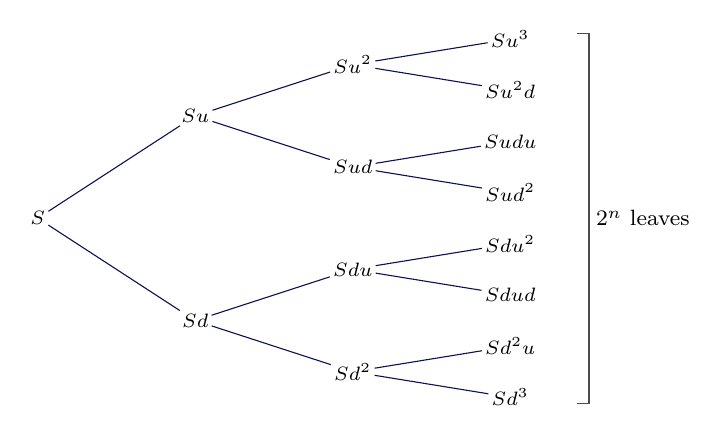
\begin{tikzpicture}[font=\scriptsize, every node/.style={inner sep=1pt},
			level distance=2.0cm,
			level 1/.style={sibling distance=2.6cm},
			level 2/.style={sibling distance=1.3cm},
			level 3/.style={sibling distance=0.65cm},
			grow=right, edge from parent/.style={draw, MidnightBlue!70!black}]
		\node {$S$}
		child {node {$Sd$}
				child {node {$Sd^{2}$} child {node {$Sd^{3}$}} child {node {$Sd^{2}u$}}}
				child {node {$Sdu$} child {node {$Sdud$}} child {node {$Sdu^{2}$}}}}
		child {node {$Su$}
				child {node {$Sud$} child {node {$Sud^{2}$}} child {node {$Sudu$}}}
				child {node {$Su^{2}$} child {node {$Su^{2}d$}} child {node {$Su^{3}$}}}};
		\draw[Gray!60!black] (6.85,2.35) -- (7.0,2.35) -- (7.0,-2.35) -- (6.85,-2.35);
		\node[font=\footnotesize, anchor=west] at (7.05,0) {$2^{n}$ leaves};
	\end{tikzpicture}
	\caption{Bushy tree：追蹤的是 path 而不是股價。像 $Su^{2}d$、$Sudu$、$Sdu^{2}$
		這些相同的股價，會以不同的 nodes 出現。}
	\label{fig:bushy}
\end{figure}

\begin{moral}
	同一個公式有三種演算法：brute-force recursion 是 $O(2^{n})$，在 recombining tree 上做 backward induction 是 $O(n^{2})$，直接對 terminal distribution 求和（\autoref{alg:bopm-optimal}）是 $O(n)$。
	第一種什麼都沒利用，第二種利用了 $ud=du$，第三種利用了 European payoff 只取決於到期時的 state --- 這也正是它不能用在 American options 的原因。
\end{moral}

%─────§ Toward Black–Scholes─────────────────────────────────────────────────────────────────────────────────────────────────────────────────────────
\section{Toward the Black--Scholes Formula}
\label{sec:toward-bs}

\source{Slides pp.~294--295}

The binomial model seems to suffer from two unrealistic assumptions:
\begin{enumerate}[(i), nosep]
	\item the stock price takes on only two values in a period;
	\item trading occurs at discrete points in time.
\end{enumerate}
As $n$ increases, however, the stock price ranges over ever larger numbers of possible values, and trading takes place nearly continuously.\footnote{Continuous-time trading may create arbitrage opportunities in practice (Budish, Cramton, \& Shim, 2015)!}
What is needed is to calibrate the BOPM's parameters $u$, $d$ and $R$ so that it converges to the continuous-time model.
We now skim through the proof.

\begin{notation}
	\begin{itemize}[nosep]
		\item $\tau$: the time to expiration of the option, measured in years;
		\item $r$: the continuously compounded \emph{annual} riskless rate;
		\item $n$: the number of periods during the option's life, so each period is $\Delta t\triangleq\tau/n$ years long.
	\end{itemize}
	The period-based quantities must then be $\hat{r}=r\tau/n=r\Delta t$ and $R=e^{\hat{r}}$.
\end{notation}

\subsection{Matching the Mean and Variance}

\source{Slides pp.~296--300}

Under the binomial model, $\ln u$ and $\ln d$ are the stock's two possible continuously compounded rates of return per period.
After $j$ up moves out of $n$,
\begin{equation}
	\ln\frac{S_{\tau}}{S} \;=\; \ln\frac{Su^{j}d^{n-j}}{S} \;=\; j\ln(u/d)+n\ln d ,
	\label{eq:bopm-log-return}
\end{equation}
where $j$ is binomial with parameters $n$ and $q$ (the \emph{true} up probability of \autoref{sec:bopm}), so $E[\,j\,]=nq$ and $\Var[\,j\,]=nq(1-q)$.

\begin{definition}
	Let
	\[
		\hat{\mu} \;\triangleq\; \frac{1}{n}\,E\left[\ln\frac{S_{\tau}}{S}\right] ,
		\qquad
		\hat{\sigma}^{2} \;\triangleq\; \frac{1}{n}\,\Var\left[\ln\frac{S_{\tau}}{S}\right]
	\]
	denote the expected value and the variance of the continuously compounded rate of return \emph{per period} of the BOPM.
\end{definition}

From \eqref{eq:bopm-log-return} it is not hard to show that
\[
	\hat{\mu} \;=\; q\ln(u/d)+\ln d ,
	\qquad
	\hat{\sigma}^{2} \;=\; q(1-q)\ln^{2}(u/d) .
\]
Indeed, each period contributes an independent Bernoulli variable equal to $\ln u$ or $\ln d$.

Assume the stock's true continuously compounded rate of return over $\tau$ years has mean $\mu\tau$ and variance $\sigma^{2}\tau$.
Call $\sigma$ the stock's (annualized) \vocab{volatility}.

\begin{remark}
	\vocab{波動率}（volatility）$\sigma$：年化的連續複利報酬率的標準差，$\tau$ 年的對數報酬變異數是 $\sigma^{2}\tau$。注意變異數與時間成正比，所以標準差與 $\sqrt{\tau}$ 成正比。
\end{remark}

The BOPM converges to that distribution only if
\begin{align}
	n\hat{\mu}      & \;=\; n\bigl[\,q\ln(u/d)+\ln d\,\bigr] \;\to\; \mu\tau ,         \label{eq:calib-mean} \\
	n\hat{\sigma}^{2} & \;=\; nq(1-q)\ln^{2}(u/d) \;\to\; \sigma^{2}\tau .           \label{eq:calib-var}
\end{align}
These are two conditions on three unknowns $u,d,q$, so we need one more.
Impose
\[
	ud \;=\; 1 .
\]
It makes nodes at the same horizontal level of the tree have identical prices (\autoref{fig:bopm-zeros}); other choices are possible.\footnote{Exact solutions for $u,d,q$ are feasible if \eqref{eq:calib-mean}--\eqref{eq:calib-var} are replaced by equations: 3 equations for 3 variables (Chance, 2008). Exercise 9.3.1 of the textbook instead imposes $q=1/2$.}

\begin{proposition}
	\label{prop:crr}
	The requirements are satisfied by
	\begin{equation}
		u \;=\; e^{\sigma\sqrt{\Delta t}} ,
		\qquad
		d \;=\; e^{-\sigma\sqrt{\Delta t}} ,
		\qquad
		q \;=\; \frac{1}{2}+\frac{1}{2}\,\frac{\mu}{\sigma}\sqrt{\Delta t} ,
		\label{eq:crr}
	\end{equation}
	for which
	\[
		n\hat{\mu} \;=\; \mu\tau ,
		\qquad
		n\hat{\sigma}^{2} \;=\; \Bigl[\,1-\Bigl(\frac{\mu}{\sigma}\Bigr)^{2}\Delta t\,\Bigr]\sigma^{2}\tau \;\to\; \sigma^{2}\tau .
	\]
\end{proposition}

\begin{proof}
	Now $\ln(u/d)=2\sigma\sqrt{\Delta t}$ and $\ln d=-\sigma\sqrt{\Delta t}$, so
	\[
		n\hat{\mu} \;=\; n\sigma\sqrt{\Delta t}\,(2q-1) \;=\; n\sigma\sqrt{\Delta t}\cdot\frac{\mu}{\sigma}\sqrt{\Delta t} \;=\; n\mu\Delta t \;=\; \mu\tau .
	\]
	For the variance, $q(1-q)=\frac14-\frac14(2q-1)^{2}=\frac14\bigl[1-(\mu/\sigma)^{2}\Delta t\bigr]$, hence
	\[
		n\hat{\sigma}^{2} \;=\; n\cdot\tfrac14\bigl[1-(\mu/\sigma)^{2}\Delta t\bigr]\cdot4\sigma^{2}\Delta t \;=\; \bigl[1-(\mu/\sigma)^{2}\Delta t\bigr]\sigma^{2}\tau .
		\qedhere
	\]
\end{proof}

With this choice, even if $\sigma$ is not calibrated correctly, the mean is still matched exactly.
Note also that $u$ and $d$ are related to volatility exclusively: both are independent of $r$ and $\mu$.
All the information about the drift sits in the probability; that is the same division of labour as in \autoref{sec:bopm-risk}, where only $u$ and $d$ entered the price.

\subsection{The CRR Model}

\source{Slides pp.~301--302}

The choices \eqref{eq:crr} result in the \vocab{CRR binomial model}.\footnote{Cox, Ross, \& Rubinstein (1979).}
Black (1992): ``This method is probably used more than the original formula in practical situations.''
OptionMetrics's (2015) IvyDB, for instance, uses the CRR model.

\begin{remark}
	\vocab{CRR 二項式模型}（Cox--Ross--Rubinstein binomial model）：取 $u=e^{\sigma\sqrt{\Delta t}}$、$d=1/u$，每期對數股價上下移動 $\sigma\sqrt{\Delta t}$；形成一個在 $\ln S$ 座標下等距的格子。$u,d$ 只由波動率決定，期望報酬只影響機率。
\end{remark}

The CRR model is best seen in logarithmic terms:
\[
	\ln S \;\longrightarrow\;
	\begin{cases}
		\ln S+\sigma\sqrt{\Delta t}, & \text{up move},   \\
		\ln S-\sigma\sqrt{\Delta t}, & \text{down move}.
	\end{cases}
\]
In the $(t,\ln S)$ plane the tree is a regular lattice (\autoref{fig:crr-lattice}).

\begin{figure}[H]
	\centering
	\begin{tikzpicture}[font=\footnotesize, x=1.3cm, y=0.72cm]
		\foreach \k in {-3,...,3} \draw[Gray!45, densely dashed] (0,\k) -- (3.3,\k);
		\foreach \t in {0,1,2,3} \draw[Gray!45, densely dashed] (\t,-3.4) -- (\t,3.4);
		\draw[-{Stealth[length=4pt]}] (0,-3.6) -- (0,3.8) node[above] {$\ln S$};
		\draw[-{Stealth[length=4pt]}] (0,-3.6) -- (3.6,-3.6) node[right] {$t$};
		\foreach \t in {0,1,2,3} \node[below] at (\t,-3.6) {$\t$};
		\foreach \t in {0,1,2,3}{
				\foreach \i in {0,...,\t}{
						\pgfmathtruncatemacro{\k}{\t-2*\i}
						\fill[MidnightBlue!80!black] (\t,\k) circle (2.3pt);
						\ifnum\t<3
							\pgfmathtruncatemacro{\kk}{\k+1}
							\pgfmathtruncatemacro{\km}{\k-1}
							\pgfmathtruncatemacro{\tn}{\t+1}
							\draw[MidnightBlue!70!black] (\t,\k) -- (\tn,\kk);
							\draw[MidnightBlue!70!black] (\t,\k) -- (\tn,\km);
						\fi
					}
			}
		\draw[|-|, Gray!60!black] (3.45,1) -- (3.45,2) node[midway, right] {$\sigma\sqrt{\Delta t}$};
		\draw[|-|, Gray!60!black] (0,-4.35) -- (1,-4.35) node[midway, below] {$\Delta t$};
	\end{tikzpicture}
	\caption{The CRR tree in logarithmic coordinates: every move is
		$\pm\sigma\sqrt{\Delta t}$, and since $ud=1$ the tree is symmetric about the
		starting level.}
	\label{fig:crr-lattice}
\end{figure}

\subsection{When the Probabilities Misbehave}

\source{Slides p.~303}

The no-arbitrage inequalities $d<R<u$ may not hold under \eqref{eq:crr} or \eqref{eq:risk-neutral-p}.
If this happens, the risk-neutral probabilities lie outside $[0,1]$.\footnote{Many papers and programs forget to check this condition!}
With $r\ge0$ the inequality $d<R$ is automatic, and $R<u$ means $e^{\sigma\sqrt{\Delta t}}>e^{r\Delta t}$, i.e., $\sigma>r\sqrt{\tau/n}$, i.e.,
\begin{equation}
	n \;>\; \frac{r^{2}}{\sigma^{2}}\,\tau .
	\label{eq:crr-n-bound}
\end{equation}
So the problem goes away if $n$ is large enough.
Other solutions can be found in the textbook\footnote{See Exercise 9.3.1 of the textbook.} or will be presented later.

\begin{eg}
	With $r=10\%$, $\sigma=5\%$ and $\tau=1$, \eqref{eq:crr-n-bound} requires $n>4$: a two-period CRR tree for a low-volatility stock has $p>1$.
	For typical equity volatilities the bound is far below $1$ and never binds.
\end{eg}

\subsection{The Limiting Distribution}

\source{Slides pp.~304--305}

By \eqref{eq:bopm-log-return}, $\ln(S_{\tau}/S)$ is a sum of $n$ independent Bernoulli variables.
The central limit theorem (\autoref{thm:clt}) therefore says $\ln(S_{\tau}/S)$ converges to $N(\mu\tau,\sigma^{2}\tau)$.\footnote{As our probabilities depend on $n$, this argument is only heuristic; the rigorous version uses the Lyapunov condition, $\bigl[(1-q)^{2}+q^{2}\bigr]/\bigl[nq(1-q)\bigr]\to0$, which holds here. See Uspensky (1937).}
So $\ln S_{\tau}$ approaches $N(\mu\tau+\ln S,\,\sigma^{2}\tau)$.

\begin{moral}
	$S_{\tau}$ has a lognormal distribution in the limit.
	This is the distribution \autoref{sec:lognormal} prepared for; the binomial tree has now \emph{derived} it, rather than assumed it.
\end{moral}

Which $\mu$?
For pricing we need the tree under the risk-neutral probability, not under $q$.

\begin{lemma}
	\label{lem:rn-lognormal}
	The continuously compounded rate of return $\ln(S_{\tau}/S)$ approaches the normal distribution with mean $(r-\sigma^{2}/2)\,\tau$ and variance $\sigma^{2}\tau$ in a risk-neutral economy.
\end{lemma}

\begin{proof}[Proof sketch]
	Let $q$ equal the risk-neutral probability $p\triangleq(e^{r\tau/n}-d)/(u-d)$ and let $n\to\infty$.
	Expanding $e^{y}=1+y+y^{2}/2+\cdots$ with $u=e^{\sigma\sqrt{\Delta t}}$, $d=e^{-\sigma\sqrt{\Delta t}}$:
	\[
		e^{r\Delta t}-d \;=\; \sigma\sqrt{\Delta t}+\Bigl(r-\frac{\sigma^{2}}{2}\Bigr)\Delta t+O\bigl(\Delta t^{3/2}\bigr) ,
		\qquad
		u-d \;=\; 2\sigma\sqrt{\Delta t}+O\bigl(\Delta t^{3/2}\bigr) ,
	\]
	so
	\[
		p \;=\; \frac12+\frac12\,\frac{r-\sigma^{2}/2}{\sigma}\sqrt{\Delta t}+O(\Delta t) .
	\]
	Comparing with $q$ in \eqref{eq:crr}, $p$ is the CRR probability with $\mu=r-\sigma^{2}/2$.\footnote{More precisely, $p=\frac12+\frac{\mu}{2\sigma}(\Delta t)^{0.5}+\frac{\sigma^{4}+4\sigma^{2}\mu+6\mu^{2}}{24\sigma}(\Delta t)^{1.5}+O\bigl(\Delta t^{2.5}\bigr)$ with $\mu=r-\sigma^{2}/2$, consistent with \eqref{eq:crr}. See Lemma 9.3.3 of the textbook.}
	\autoref{prop:crr} and the central limit theorem then give the claim.
\end{proof}

\begin{remark}
	這就是 \autoref{sec:lognormal} 預告的「$-\sigma^{2}/2$ 修正項」：在風險中立世界裡，股價的\emph{期望}成長率要是 $r$，所以對數報酬的平均只能是 $r-\sigma^{2}/2$，多出來的 $\sigma^{2}/2$ 由 Jensen 不等式（\autoref{thm:jensen}）補回。
\end{remark}

\subsection{Two Meanings of ``Rate of Return''}

\source{Slides pp.~306--307}

The expected stock price at expiration in a risk-neutral economy is $Se^{r\tau}$, by \autoref{lem:rn-lognormal} and \eqref{eq:lognormal-moments}:
\[
	E\bigl[\,S_{\tau}\,\bigr] \;=\; S\exp\Bigl[\Bigl(r-\frac{\sigma^{2}}{2}\Bigr)\tau+\frac{\sigma^{2}\tau}{2}\Bigr] \;=\; Se^{r\tau} .
\]
So the stock's expected annual rate of return is the riskless rate $r$ --- \emph{if} the rate of return means
\[
	\frac{\ln E\bigl[\,S_{\tau}/S\,\bigr]}{\tau} ,
\]
the (weighted) arithmetic average rate of return, annualized.
If it means instead
\[
	\frac{E\bigl[\,\ln(S_{\tau}/S)\,\bigr]}{\tau} ,
\]
the (weighted) geometric average rate of return, annualized, then \autoref{lem:rn-lognormal} gives $r-\sigma^{2}/2$.

\begin{note}
	這兩個敘述同時成立，因為它們回答的是不同的問題。
	第一個講的是各情境下 \emph{wealth} 的平均，第二個講的是單一情境中典型（median）的 \emph{growth}。
	Jensen's inequality（\autoref{thm:jensen}）讓第二個小於第一個，對 lognormal 而言剛好差 $\sigma^{2}/2$。
\end{note}

\subsection{The Black--Scholes Formula}
\label{sec:black-scholes}

\source{Slides p.~308}

\begin{theorem}[The Black--Scholes Formula, 1973]
	\label{thm:black-scholes}
	\begin{align}
		C & \;=\; SN(x)-Xe^{-r\tau}N\bigl(x-\sigma\sqrt{\tau}\bigr) , \label{eq:bs-call} \\
		P & \;=\; Xe^{-r\tau}N\bigl(-x+\sigma\sqrt{\tau}\bigr)-SN(-x) , \label{eq:bs-put}
	\end{align}
	where
	\begin{equation}
		x \;\triangleq\; \frac{\ln(S/X)+\bigl(r+\sigma^{2}/2\bigr)\tau}{\sigma\sqrt{\tau}} .
		\label{eq:bs-x}
	\end{equation}
\end{theorem}

On a United flight from San Francisco to Tokyo on March 7, 2010, a real-estate manager mentioned this formula to the lecturer!

\begin{proof}
	By \eqref{eq:rn-pricing} in the limit, $C=e^{-r\tau}E^{\pi}\bigl[\max(S_{\tau}-X,0)\bigr]$, and by \autoref{lem:rn-lognormal} $\ln S_{\tau}\sim N(m,s^{2})$ under $\pi$ with
	\[
		m \;=\; \ln S+\Bigl(r-\frac{\sigma^{2}}{2}\Bigr)\tau ,
		\qquad
		s \;=\; \sigma\sqrt{\tau} .
	\]
	This is precisely the setting of \autoref{cor:lognormal-call} with $a=X$.
	There $e^{m+s^{2}/2}=Se^{r\tau}$, and
	\[
		d_{2} \;=\; \frac{m-\ln X}{s} \;=\; \frac{\ln(S/X)+(r-\sigma^{2}/2)\tau}{\sigma\sqrt{\tau}} \;=\; x-\sigma\sqrt{\tau} ,
		\qquad
		d_{1} \;=\; d_{2}+s \;=\; x .
	\]
	So \eqref{eq:lognormal-call} gives $E^{\pi}\bigl[\max(S_{\tau}-X,0)\bigr]=Se^{r\tau}N(x)-XN(x-\sigma\sqrt{\tau})$; multiplying by $e^{-r\tau}$ yields \eqref{eq:bs-call}.

	For the put, use put--call parity (\autoref{thm:put-call-parity}) with $\mathrm{PV}(X)=Xe^{-r\tau}$ and $1-N(z)=N(-z)$:
	\[
		P \;=\; C-S+Xe^{-r\tau} \;=\; Xe^{-r\tau}\bigl[1-N(x-\sigma\sqrt{\tau})\bigr]-S\bigl[1-N(x)\bigr] ,
	\]
	which is \eqref{eq:bs-put}.
\end{proof}

\begin{note}
	上面的證明是先對\emph{分布}取極限再定價；課本則反過來，直接對 \eqref{eq:bopm-formula} 取極限。\footnote{課本 Theorem 9.3.4。}
	那裡同樣用 central limit theorem 證明兩個 binomial 尾端和會收斂：
	\[
		\sum_{j=a}^{n}b\bigl(j;n,pu/R\bigr)\;\to\;N(x) ,
		\qquad
		\sum_{j=a}^{n}b(j;n,p)\;\to\;N\bigl(x-\sigma\sqrt{\tau}\bigr) .
	\]
	不論哪種做法，得到的公式都是 \eqref{eq:bopm-formula} 之後提到的那個形狀。
\end{note}

\begin{remark}
	\vocab{Black--Scholes 公式}：$C=SN(x)-Xe^{-r\tau}N(x-\sigma\sqrt{\tau})$。只需要五個輸入 $S,X,\sigma,\tau,r$；股票的期望報酬 $\mu$ 不出現，正如 \autoref{sec:bopm-risk} 中 $q$ 不出現一樣。
\end{remark}

\subsection{Interpreting \texorpdfstring{$N(x)$}{N(x)} and \texorpdfstring{$N(x-\sigma\sqrt{\tau})$}{N(x - sigma sqrt tau)}}
\label{sec:bs-interpret}

\source{Slides p.~309}

Compare \eqref{eq:bs-call} with \eqref{eq:bopm-formula} for the meaning of $x$.
\begin{itemize}[itemsep=0.3em]
	\item $N(x-\sigma\sqrt{\tau})$ is the limit of $\sum_{j\ge a}b(j;n,p)$: the risk-neutral probability that the call finishes in the money, $\mathrm{Prob}^{\pi}[\,S_{\tau}>X\,]$ (cf.\ \autoref{prop:lognormal-tail}).
	\item $N(x)$ is the limit of $\sum_{j\ge a}b(j;n,pu/R)$: the probability of the same event under the tilted measure $pu/R$, which weights each path by how much the stock grew along it.\footnote{See Exercise 13.2.12 of the textbook for an interpretation of the probability associated with $N(x)$ and $N(-x)$.}
\end{itemize}

\begin{eg}
	\label{eg:bs-binary}
	The binary call of \autoref{sec:binary-call} pays \$1 exactly when $S_{\tau}>X$, so under Black--Scholes its price is
	\[
		e^{-r\tau}\,\mathrm{Prob}^{\pi}[\,S_{\tau}>X\,] \;=\; e^{-r\tau}N\bigl(x-\sigma\sqrt{\tau}\bigr) .
	\]
	The model-free formula \eqref{eq:binary-call} agrees: differentiating \eqref{eq:bs-call} in $X$, the terms containing $N'$ cancel by \eqref{eq:bs-identity} below, and $-\partial C/\partial X=e^{-r\tau}N(x-\sigma\sqrt{\tau})$.\footnote{Exercise 9.3.5 of the textbook.}
\end{eg}

%─────§ BOPM and BS──────────────────────────────────────────────────────────────────────────────────────────────────────────────────────────────────
\section{BOPM and Black--Scholes Model}
\label{sec:bopm-vs-bs}

\source{Slides p.~310}

The Black--Scholes formula needs 5 parameters: $S$, $X$, $\sigma$, $\tau$ and $r$.
Binomial tree algorithms take 6 inputs: $S$, $X$, $u$, $d$, $\hat{r}$ and $n$.
The connections are
\[
	u \;=\; e^{\sigma\sqrt{\tau/n}} ,
	\qquad
	d \;=\; e^{-\sigma\sqrt{\tau/n}} ,
	\qquad
	\hat{r} \;=\; r\tau/n ,
\]
which is the CRR model \eqref{eq:crr} again.

\begin{eg}
	Consider a 3-month option when the interest rate is 8\% per annum and the volatility is 30\% per annum, so $\tau=0.25$, $r=0.08$ and $\sigma=0.3$.
	A binomial tree with $n=5$ should use $u=e^{0.3\sqrt{0.25/5}}=1.0694$, $d=e^{-0.3\sqrt{0.25/5}}=0.9351$ and $\hat{r}=0.004$.\footnote{Example 9.3.5 of the textbook.}
\end{eg}

\source{Slides pp.~311--312}

\begin{figure}[H]
	\centering
	\begin{tikzpicture}[font=\footnotesize]
		\begin{groupplot}[
				group style={group size=2 by 1, horizontal sep=1.5cm},
				width=0.48\textwidth, height=5.0cm,
				xlabel={$n$},
				title style={font=\small, text=Gray!40!black},
				tick label style={font=\scriptsize},
				label style={font=\scriptsize},
				yticklabel style={/pgf/number format/fixed, /pgf/number format/precision=1},
				axis line style={thin}, tick align=outside,
			]
			\nextgroupplot[title={Call value, $X=100$}, xmin=0, xmax=36, ymin=11.1, ymax=13.5]
			\addplot[Gray!60, densely dashed, thick] coordinates {(0,12.1058) (36,12.1058)};
			\addplot[MidnightBlue!80!black, thin, mark=*, mark size=0.9pt] coordinates {
					(1,13.4278) (2,11.1739) (3,12.5944) (4,11.6142) (5,12.4012) (6,11.7730) (7,12.3170) (8,11.8544) (9,12.2701) (10,11.9039) (11,12.2402) (12,11.9371) (13,12.2195) (14,11.9610) (15,12.2043) (16,11.9789) (17,12.1927) (18,11.9929) (19,12.1835) (20,12.0041) (21,12.1761) (22,12.0133) (23,12.1700) (24,12.0210) (25,12.1649) (26,12.0275) (27,12.1605) (28,12.0330) (29,12.1567) (30,12.0379) (31,12.1534) (32,12.0421) (33,12.1505) (34,12.0458) (35,12.1480)};
			\nextgroupplot[title={Call value, $X=95$}, xmin=0, xmax=61, ymin=15.0, ymax=15.55,
				yticklabel style={/pgf/number format/precision=2}]
			\addplot[Gray!60, densely dashed, thick] coordinates {(0,15.1749) (61,15.1749)};
			\addplot[RawSienna, thin, mark=*, mark size=0.8pt] coordinates {
					(1,16.4603) (2,15.0821) (3,15.5047) (4,15.2692) (5,15.2877) (6,15.2981) (7,15.1935) (8,15.2974) (9,15.1411) (10,15.2891) (11,15.1077) (12,15.2787) (13,15.0846) (14,15.2681) (15,15.0676) (16,15.2581) (17,15.0950) (18,15.2487) (19,15.1192) (20,15.2400) (21,15.1376) (22,15.2319) (23,15.1516) (24,15.2245) (25,15.1626) (26,15.2177) (27,15.1711) (28,15.2113) (29,15.1778) (30,15.2054) (31,15.1831) (32,15.1998) (33,15.1872) (34,15.1947) (35,15.1904) (36,15.1898) (37,15.1929) (38,15.1853) (39,15.1948) (40,15.1810) (41,15.1963) (42,15.1769) (43,15.1973) (44,15.1731) (45,15.1980) (46,15.1695) (47,15.1984) (48,15.1660) (49,15.1986) (50,15.1628) (51,15.1986) (52,15.1596) (53,15.1984) (54,15.1567) (55,15.1981) (56,15.1538) (57,15.1977) (58,15.1511) (59,15.1972) (60,15.1485)};
		\end{groupplot}
	\end{tikzpicture}
	\caption{CRR binomial call values against the number of periods $n$, with
		$S=100$, $r=8\%$, $\sigma=0.2$, $\tau=1$. Dashed: the Black--Scholes values
		$12.1058$ (left) and $15.1749$ (right). The value at $n=1$ on the right
		($16.46$) is off the scale.}
	\label{fig:bopm-convergence}
\end{figure}

The binomial tree algorithms converge reasonably fast: the error is $O(1/n)$.\footnote{F.~Diener \& M.~Diener (2004); L.~Chang \& Palmer (2007).}
Oscillations are inherent, however, and they can be dealt with by judicious choices of $u$ and $d$.\footnote{See Exercise 9.3.8 of the textbook, which shifts the lattice by $(1/n)\ln(X/S)$ so that the strike always falls on a node.}

\begin{intuition}
	The oscillation comes from where the strike falls on the terminal lattice.
	At the money ($X=S$, left), the middle terminal node sits exactly at $X$ for even $n$ and the two nearest straddle it for odd $n$, which flips the error's sign each step --- hence the saw-tooth.
	For $X=95$ (right) the strike's position relative to the nodes drifts slowly with $n$, producing the longer, irregular waves.
	The $\max(\cdot,0)$ kink is the only thing the lattice resolves badly; that is also the moral of \autoref{sec:numerical-gamma-fails}.
	Barrier options make the misplacement much worse (\autoref{fig:barrier-convergence}).
\end{intuition}

%─────§ Implied volatility──────────────────────────────────────────────────────────────────────────────────────────────────────────────────────────
\section{Implied Volatility}
\label{sec:implied-vol}

\source{Slides pp.~313--314}

Of the five inputs, volatility is the sole parameter not directly observable.
The Black--Scholes formula can be used to compute the market's opinion of it: solve for $\sigma$ given the option price, $S$, $X$, $\tau$ and $r$, with the numerical methods of \autoref{sec:numerical-irr}.
The result is the \vocab{implied volatility}.

\begin{remark}
	\vocab{隱含波動率}（implied volatility）：把市場上的選擇權價格代回 Black--Scholes 公式反解出來的 $\sigma$，可以看成市場對未來波動的「共識」。跟它相對的是\vocab{歷史波動率}（historical volatility），由過去股價的對數報酬估計。
\end{remark}

\begin{note}
	根存在且唯一，因為 call 價格對 $\sigma$ 嚴格遞增 --- 它的 vega 為正（\autoref{sec:vega}）--- 而且 $\sigma\to0$ 時趨近 $\max(S-Xe^{-r\tau},0)$，$\sigma\to\infty$ 時趨近 $S$。
	這裡很自然用 Newton--Raphson，以 vega 作為 $f'$。
	投影片上的兩個問題：
	\begin{itemize}[nosep]
		\item \emph{American options 呢？} 沒有公式可以反解，所以每一步 Newton 都要用 tree 定價；如果改用 European 公式反解，會高估 volatility，因為 early-exercise premium 被算到 $\sigma$ 頭上。\footnote{課本 Exercise 9.4.2。}
		\item \emph{為什麼 $\tau$ 很小時很難？} 因為 $\tau\to0$ 時 vega 趨近零（\autoref{sec:vega}）：價格幾乎不隨 $\sigma$ 變動，所以價格上一點點誤差就會讓 implied $\sigma$ 大幅移動。
	\end{itemize}
\end{note}

Implied volatility is
\begin{quote}
	\itshape the wrong number to put in the wrong formula to get the right price of plain-vanilla options.\footnote{Rebonato (2004).}
\end{quote}
Think of it as an alternative to quoting option prices.
It is often preferred to historical (statistical) volatility in practice.
Is using the historical volatility like driving a car with your eyes on the rearview mirror?\footnote{E.g., 1:16:23 of \url{https://www.youtube.com/watch?v=8TJQhQ2GZ0Y}.}
Note that volatility is meaningful only if seen through a model!\footnote{Alexander (2001).}

\subsection{Problems; the Smile}

\source{Slides pp.~315--318}

Options written on the same underlying asset usually do not yield the same implied volatility.
A typical pattern is a \vocab{smile} in relation to the strike price:\footnote{Alexander (2001).}
the implied volatility is lowest for at-the-money options and becomes higher the further the option is in- or out-of-the-money.
This is common for foreign exchange options.

Other patterns have also been observed.
For stock options, low-strike options tend to have higher implied volatilities (a \vocab{skew}).
\begin{itemize}[nosep]
	\item One explanation is the high demand for insurance provided by out-of-the-money puts.
	\item Another is that volatility rises when the stock falls,\footnote{This is called the \vocab{leverage effect} (Black, 1992).} making in-the-money calls more likely to become in the money again.
\end{itemize}

\begin{remark}
	\vocab{波動率微笑}（volatility smile）：同一標的、同一到期日，不同履約價的隱含波動率畫出來像笑臉，價平最低、兩端翹起（外匯選擇權常見）。股票選擇權則多半是\vocab{波動率偏斜}（skew）：低履約價的隱含波動率較高。若 Black--Scholes 完全正確，這條線應該是水平的。
\end{remark}

\begin{figure}[H]
	\centering
	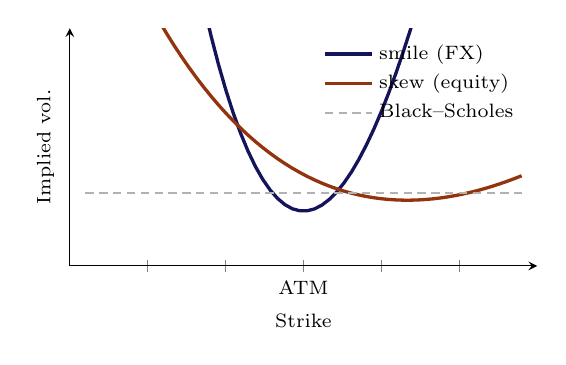
\begin{tikzpicture}[font=\footnotesize]
		\begin{axis}[
				width=0.62\textwidth, height=4.6cm,
				xmin=70, xmax=130, ymin=12, ymax=38,
				xtick={80,90,100,110,120}, xticklabels={,,ATM,,},
				ytick=\empty,
				xlabel={Strike}, ylabel={Implied vol.},
				axis lines=left, axis line style={thin},
				label style={font=\scriptsize}, tick label style={font=\scriptsize},
				legend style={font=\scriptsize, draw=none, fill=none, at={(0.98,0.98)}, anchor=north east},
				legend cell align=left,
			]
			\addplot[MidnightBlue!80!black, very thick, domain=72:128, samples=60] {18+1200*(ln(x/100))^2};
			\addlegendentry{smile (FX)}
			\addplot[RawSienna, very thick, domain=72:128, samples=60] {22-45*ln(x/100)+180*(ln(x/100))^2};
			\addlegendentry{skew (equity)}
			\addplot[Gray!60, densely dashed, thick] coordinates {(72,20) (128,20)};
			\addlegendentry{Black--Scholes}
		\end{axis}
	\end{tikzpicture}
	\caption{Schematic shapes of implied volatility against strike. The slides
		show real data for TXO calls on September 25, 2015 (TAIEX closed at 8132),
		where implied volatility ranged from about 14\% to 24\% across strikes and
		maturities.}
	\label{fig:smile}
\end{figure}

To address this issue, volatilities are often combined to produce a composite implied volatility.
This practice is not sound theoretically.
The existence of different implied volatilities for options on the same underlying asset shows the Black--Scholes model is not literally true.

\begin{moral}
	A single stock has a single volatility in the Black--Scholes model, so the smile is a measurement of the model's error, not of the stock.
	By \autoref{thm:breeden-litzenberger}, a non-flat smile is the market telling us its risk-neutral density of $S_{\tau}$ is \emph{not} lognormal --- typically with fatter tails, exactly as \autoref{fig:sp500-density} showed for realized returns.
\end{moral}

%─────§ American puts──────────────────────────────────────────────────────────────────────────────────────────────────────────────────────────────
\section{Binomial Tree Algorithms for American Puts}
\label{sec:american-puts}

\source{Slides p.~319}

Early exercise has to be considered.
The binomial tree algorithm starts with the terminal payoffs $\max\bigl(0,\,X-Su^{j}d^{n-j}\bigr)$ and applies backward induction.
At each intermediate node, compare the payoff if exercised and the continuation value, and keep the larger one.

\begin{algorithm}[H]
	\caption{Binomial tree algorithm for American puts on a non-dividend-paying stock}
	\label{alg:american-put}
	\KwIn{$S,u,d,X,n,\hat{r}$ \quad ($u>e^{\hat{r}}>d$)}
	$R:=e^{\hat{r}}$\;
	$p:=(R-d)/(u-d)$\;
	\For{$i=0,1,\ldots,n$}{
		$P[\,i\,]:=\max\bigl(0,\,X-Su^{n-i}d^{i}\bigr)$\;
	}
	\For{$j=n-1$ \KwTo $0$}{
		\For{$i=0,1,\ldots,j$}{
			$P[\,i\,]:=\max\Bigl(\bigl(p\times P[\,i\,]+(1-p)\times P[\,i+1\,]\bigr)/R,\ X-Su^{j-i}d^{i}\Bigr)$\;
		}
	}
	\Return{$P[\,0\,]$}\;
\end{algorithm}

\begin{eg}
	\label{eg:american-put}
	Take the tree of \autoref{eg:bopm-three-period} ($S=160$, $u=1.5$, $d=0.5$, $R=1.2$, $p=0.7$) with an American put struck at $X=130$.\footnote{The numerical example in Section 9.5 of the textbook.}
	At time~2, the node $S=120$ has continuation value $(0.7\times0+0.3\times70)/1.2=17.5$, greater than the intrinsic value $130-120=10$: the put is in the money but should \emph{not} be exercised.
	The node $S=40$ has continuation value $(0.7\times70+0.3\times110)/1.2=68.33$, lower than the intrinsic value $130-40=90$: exercise.
	Continuing, the node $S=80$ at time~1 is also exercised ($50$ against a continuation value of $32.71$), and the American put is worth
	\[
		\frac{0.7\times4.375+0.3\times50}{1.2} \;=\; 15.05 ,
	\]
	against $9.375$ for the European put.
\end{eg}

\subsection{Bermudan Options}

\source{Slides p.~320}

Some American options can be exercised only at discrete time points instead of continuously.
They are called \vocab{Bermudan options}.
Their pricing algorithm is identical to that for American options, but early exercise is considered for only those nodes when early exercise is permitted.

\begin{remark}
	\vocab{百慕達式選擇權}（Bermudan option）：只能在事先約定的幾個日期提前履約，介於歐式（只能到期履約）與美式（隨時可履約）之間——就像百慕達在地理上介於歐洲與美國之間。演算法上只在允許履約的那幾欄取 $\max$。
\end{remark}

%─────§ Time-dependent parameters───────────────────────────────────────────────────────────────────────────────────────────────────────────────────
\section{Time-Dependent Parameters}
\label{sec:time-dependent}

\subsection{Time-Dependent Volatility}

\source{Slides pp.~321--323}

Suppose the (instantaneous) volatility can change over time but is otherwise predictable: $\sigma(t)$ instead of $\sigma$.\footnote{Merton (1973).}
Variances of independent increments add, so in the limit the variance of $\ln(S_{\tau}/S)$ is
\[
	\int_{0}^{\tau}\sigma^{2}(t)\,dt
\]
rather than $\sigma^{2}\tau$.
The annualized volatility to be used in the Black--Scholes formula should now be
\[
	\sqrt{\frac{\int_{0}^{\tau}\sigma^{2}(t)\,dt}{\tau}} ,
\]
the root-mean-square of $\sigma(t)$ --- \emph{not} its average.

For the binomial model, $u$ and $d$ now depend on time:
\[
	u \;=\; e^{\sigma(t)\sqrt{\tau/n}} ,
	\qquad
	d \;=\; e^{-\sigma(t)\sqrt{\tau/n}} .
\]
But then the tree no longer combines: an up move at time $t_{1}$ followed by a down move at $t_{2}$ multiplies the price by $e^{(\sigma(t_{1})-\sigma(t_{2}))\sqrt{\Delta t}}$, and the reverse order by its reciprocal.\footnote{Amin (1991); C.~I.~Chen (\texttt{R98922127}) (2011).}
One way out is to let the period lengths vary so that $\sigma(t_{i})\sqrt{\Delta t_{i}}$ stays constant; then every period moves $\ln S$ by the same $\pm$ step and the lattice is regular again.

The CBOE S\&P 500 Volatility Index (\vocab{VIX}) tracks the 30-day implied volatility of S\&P 500 index options; its history over 1990--2016 (plotted on the slides) shows how far from constant volatility actually is, with spikes above 80 during the 2008 crisis.

\subsection{Time-Dependent Short Rates}

\source{Slides p.~324}

Suppose the short rate (i.e., the one-period spot rate or forward rate) changes over time but predictably.
The annual riskless rate $r$ in the Black--Scholes formula should be the spot rate with a time to maturity equal to $\tau$.
In other words,
\[
	r \;=\; \frac{\sum_{i=0}^{n-1}r_{i}}{\tau} ,
\]
where $r_{i}$ is the continuously compounded short rate measured in periods for period $i$, i.e., the one-period forward rate.

This is \eqref{eq:cc-avg} again: the zero-coupon bond maturing at expiration is worth $\exp\bigl(-\sum_{i}r_{i}\bigr)$ per dollar, so it carries all the interest-rate information the European option needs.

\begin{note}
	binomial tree 會不會因此不再 combine？
	不會。
	short rate 只透過 $R_{i}=e^{r_{i}}$ 進入 $p_{i}=(R_{i}-d)/(u-d)$；由 $u$ 和 $d$ 建出的價格 lattice 完全不受影響。
	backward induction 只要在第 $i$ 期改用 $p_{i}$ 和 $R_{i}$ 即可 --- 前提是每一期都滿足 $d<R_{i}<u$。
\end{note}

\subsection{Trading Days and Calendar Days}

\source{Slides pp.~325--327}

Interest accrues based on the calendar day, but $\sigma$ is usually calculated based on trading days only: stock prices seem to have lower volatilities when the exchange is closed.\footnote{Fama (1965); K.~French (1980); K.~French \& Roll (1986).}
How to harmonize these two different times in the Black--Scholes formula and binomial tree algorithms?\footnote{Recall \autoref{sec:day-count} about dating issues.}

Think of $\sigma$ as measuring the annualized volatility of stock price one year from now, and suppose a year has $m$ (say 253) trading days.
Variance accumulates only on trading days, so the variance up to expiration is $\sigma^{2}\times(\text{trading days to expiration})/m$.
Writing this in calendar time, as $\sigma_{\mathrm{eff}}^{2}\times(\text{calendar days to expiration})/365$, we can replace $\sigma$ in the Black--Scholes formula with\footnote{D.~French (1984).}
\[
	\sigma_{\mathrm{eff}} \;=\; \sigma\sqrt{\frac{365}{m}\times\frac{\text{number of trading days to expiration}}{\text{number of calendar days to expiration}}} .
\]

This works only for European options.
How about binomial tree algorithms?\footnote{Contributed by Mr.~Lu, Zheng-Liang (\texttt{D00922011}) in 2015.}
One natural answer: let each period be one trading day, with the stock moving $\pm\sigma/\sqrt{m}$ in logarithm, but discount each period over its calendar length --- three days of interest for the period spanning a weekend.
Since only $p$ and $R$ change from period to period, the tree still combines, by the previous subsection.

%─────§ Dividends──────────────────────────────────────────────────────────────────────────────────────────────────────────────────────────────────
\section{Options on a Stock That Pays Dividends}
\label{sec:dividends-tree}

\source{Slides p.~328}

Early exercise must be considered: by \autoref{thm:merton-dividend}, an American call may now be exercised just before an ex-dividend date.
The \vocab{proportional dividend payout model}, in which the dividend amount is a constant proportion of the prevailing stock price, is tractable: the price goes from $S$ to $Su(1-\delta)$ or $Sd(1-\delta)$ in a period containing an ex-dividend date, and the tree still combines.\footnote{See Sections 9.6.1--9.6.2 of the textbook.}
In general, however, the corporate dividend policy is a complex issue.

\subsection{Known Dividends}

\source{Slides pp.~329--330}

Constant dividends introduce complications.
Use $D$ to denote the amount of the dividend, and suppose an ex-dividend date falls in the first period.
At the end of that period, the possible stock prices are $Su-D$ and $Sd-D$.
Follow the stock price one more period: the number of possible stock prices is not three but four,
\[
	(Su-D)\,u ,\quad (Su-D)\,d ,\quad (Sd-D)\,u ,\quad (Sd-D)\,d .
\]
The binomial tree no longer combines, because $(Su-D)\,d\ne(Sd-D)\,u$ --- the timing of the dividend now matters.
With $m$ ex-dividend dates the number of terminal nodes is at least $2^{m}$.

\begin{figure}[H]
	\centering
	\begin{tikzpicture}[font=\small, >={Stealth[length=4pt]},
			every node/.style={inner sep=1.5pt},
			up/.style={->, MidnightBlue!75!black, shorten >=2pt, shorten <=2pt},
			dn/.style={->, RawSienna, shorten >=2pt, shorten <=2pt}]
		\begin{scope}
			\node[font=\footnotesize\bfseries, text=Gray!40!black] at (2.3,2.3) {Known dividend};
			\node (s) at (0,0) {$S$};
			\node (u) at (2.0,1.0) {$Su-D$};
			\node (d) at (2.0,-1.0) {$Sd-D$};
			\node[anchor=west] (uu) at (3.6,1.6) {$(Su-D)\,u$};
			\node[anchor=west] (ud) at (3.6,0.55) {$(Su-D)\,d$};
			\node[anchor=west] (du) at (3.6,-0.55) {$(Sd-D)\,u$};
			\node[anchor=west] (dd) at (3.6,-1.6) {$(Sd-D)\,d$};
			\draw[up] (s)--(u); \draw[dn] (s)--(d);
			\draw[up] (u)--(uu.west); \draw[dn] (u)--(ud.west);
			\draw[up] (d)--(du.west); \draw[dn] (d)--(dd.west);
		\end{scope}
		\begin{scope}[xshift=7.4cm]
			\node[font=\footnotesize\bfseries, text=Gray!40!black] at (2.3,2.3) {Ad hoc approximation};
			\node (s) at (0,0) {$S$};
			\node (u) at (2.0,1.0) {$(S-D/R)\,u$};
			\node (d) at (2.0,-1.0) {$(S-D/R)\,d$};
			\node[anchor=west] (uu) at (3.6,1.8) {$(S-D/R)\,u^{2}$};
			\node[anchor=west] (ud) at (3.6,0) {$(S-D/R)\,ud$};
			\node[anchor=west] (dd) at (3.6,-1.8) {$(S-D/R)\,d^{2}$};
			\draw[up] (s)--(u); \draw[dn] (s)--(d);
			\draw[up] (u)--(uu.west); \draw[dn] (u)--(ud.west);
			\draw[up] (d)--(ud.west); \draw[dn] (d)--(dd.west);
		\end{scope}
	\end{tikzpicture}
	\caption{Left: a known dividend $D$ paid in the first period splits the tree
		into four terminal prices. Right: the ad hoc approximation of
		\autoref{sec:adhoc-dividend}, after the PV of the dividend has been added
		back at the root (by time~1 the dividend has been paid, so nothing is
		added back there). It recombines, but with a narrower range.}
	\label{fig:dividend-trees}
\end{figure}

\subsection{An Ad-Hoc Approximation}
\label{sec:adhoc-dividend}

\source{Slides pp.~331--337}

Use the Black--Scholes formula with the stock price reduced by the PV of the dividends.\footnote{Roll (1977); Heath \& Jarrow (1988).}
This essentially decomposes the stock price into a riskless one paying known dividends and a risky one:
\begin{itemize}[nosep]
	\item the riskless component at any time is the PV of future dividends during the life of the option;
	\item $\sigma$ is the volatility of the process followed by the risky component.
\end{itemize}
The stock price, between two adjacent ex-dividend dates, follows the same lognormal distribution.

On a tree this becomes three steps:
\begin{enumerate}[(1), nosep]
	\item start with the current stock price minus the PV of future dividends before expiration;
	\item develop the binomial tree for the new stock price as if there were no dividends;
	\item add back to each stock price on the tree the PV of all future dividends before expiration.
\end{enumerate}
American option prices can be computed as before on this tree of stock prices, checking early exercise at each node.

The trees are different (\autoref{fig:dividend-trees}), and so are the stock prices at maturity: $(Su-D)u,\ (Su-D)d,\ (Sd-D)u,\ (Sd-D)d$ against $(S-D/R)u^{2},\ (S-D/R)ud,\ (S-D/R)d^{2}$.\footnote{Contributed by Mr.~Yang, Jui-Chung (\texttt{D97723002}) on March 18, 2009.}
Note that, as $d<R<u$,
\begin{align*}
	(Su-D)\,u-(S-D/R)\,u^{2} & \;=\; Du\Bigl(\frac{u}{R}-1\Bigr) \;>\; 0 , \\
	(Sd-D)\,d-(S-D/R)\,d^{2} & \;=\; Dd\Bigl(\frac{d}{R}-1\Bigr) \;<\; 0 .
\end{align*}
So the ad hoc approximation has a smaller dynamic range.
This explains why in practice the volatility is usually increased when using it.

\begin{remark}
	\textbf{為什麼範圍比較小？}
	真實的樹中，股利 $D$ 是在第一期結束時才扣掉的「固定金額」，之後的漲跌只作用在扣完的價格上；近似法則一開始就把股利的現值 $D/R$ 拿掉，讓\emph{整段}隨機成長都只作用在比較小的 $S-D/R$ 上。上漲路徑因此漲得較少、下跌路徑跌得較少，分佈被壓縮——要用較大的 $\sigma$ 補回來。
\end{remark}

\paragraph{A general approach.}
A new tree structure handles known dividends with no approximation assumptions, together with a mathematical proof that the tree can always be constructed.\footnote{T.~Dai (\texttt{B82506025}, \texttt{R86526008}, \texttt{D8852600}) \& Lyuu (2004). Also Arealy \& Rodrigues (2013).}
Its actual performance is quadratic except in pathological cases.
Other approaches include adjusting $\sigma$ and approximating the known dividend with a dividend yield.\footnote{Geske \& Shastri (1985). It works well for American options but not European ones (T.~Dai, 2009).}

\subsection{Continuous Dividend Yields}
\label{sec:continuous-yield}

\source{Slides pp.~338--339}

In the \vocab{continuous-payout model}, dividends are paid continuously.
This approximates a broad-based stock market portfolio, in which some company pays a dividend nearly every day.
The payment of a continuous dividend yield at rate $q$ reduces the growth rate of the stock price by $q$: a stock that grows from $S$ to $S_{\tau}$ with a continuous dividend yield of $q$ would have grown from $S$ to $S_{\tau}e^{q\tau}$ without the dividends.

So a European option has the same value as one on a stock with price $Se^{-q\tau}$ that pays no dividends --- in pricing European options, only the distribution of $S_{\tau}$ matters.
The Black--Scholes formulas thus hold with $S$ replaced by $Se^{-q\tau}$:\footnote{Merton (1973).}
\begin{align}
	C & \;=\; Se^{-q\tau}N(x)-Xe^{-r\tau}N\bigl(x-\sigma\sqrt{\tau}\bigr) , \label{eq:bs-call-q} \\
	P & \;=\; Xe^{-r\tau}N\bigl(-x+\sigma\sqrt{\tau}\bigr)-Se^{-q\tau}N(-x) , \label{eq:bs-put-q}
\end{align}
where now
\begin{equation}
	x \;\triangleq\; \frac{\ln(S/X)+\bigl(r-q+\sigma^{2}/2\bigr)\tau}{\sigma\sqrt{\tau}} .
	\label{eq:bs-x-q}
\end{equation}
Formulas \eqref{eq:bs-call-q} and \eqref{eq:bs-put-q} remain valid as long as the dividend yield is predictable, with $q$ the average annualized yield over the option's life.
A foreign currency is the prime example, with $q$ the foreign interest rate (\autoref{sec:forex}).

\begin{remark}
	\vocab{連續股利殖利率}（continuous dividend yield）$q$：假設股利以價格的固定比例 $q$ 連續發放，股價的成長率因而少了 $q$。對歐式選擇權來說，等同把今天的股價換成 $Se^{-q\tau}$（扣掉存續期間所有股利的「現值」）後套用原公式。
\end{remark}

\source{Slides pp.~340--341}

To run binomial tree algorithms there are two equivalent-in-spirit options, both resting on the fact that the stock price grows at an expected rate of $r-q$ in a risk-neutral economy.
\begin{enumerate}[(1), itemsep=0.3em]
	\item Replace $u$ with $ue^{-q\Delta t}$ and $d$ with $de^{-q\Delta t}$, where $\Delta t=\tau/n$; other than this, the algorithm stays the same --- in particular, $p$ should use the \emph{original} $u$ and $d$!\footnote{Contributed by Ms.~Wang, Chuan-Ju (\texttt{F95922018}) on May 2, 2007.}
	\item Keep $u$ and $d$ unchanged, but pick the risk-neutral probability as
	      \begin{equation}
		      p \;=\; \frac{e^{(r-q)\Delta t}-d}{u-d} .
		      \label{eq:rn-p-yield}
	      \end{equation}
\end{enumerate}
Either way $E^{\pi}\bigl[\,S_{t+\Delta t}\,\bigr]=Se^{(r-q)\Delta t}$: in (1), $p\,ue^{-q\Delta t}+(1-p)\,de^{-q\Delta t}=Re^{-q\Delta t}$ by \eqref{eq:rn-stock}; in (2) it is the definition of $p$.

\begin{note}
	為什麼 (1) 裡的 $p$ 必須用原本的 $u,d$？
	持有股票的人拿到的是股價\emph{加上} dividend，在 $p$ 之下必須賺到 $R$ 的是這個 total return。
	total return 是 $u$ 或 $d$；ex-dividend 價格則是 $ue^{-q\Delta t}$ 或 $de^{-q\Delta t}$。
	若用縮小後的乘數算 $p$，就等於讓 ex-dividend 價格本身賺到 $R$，也就是投資人除了 riskless rate 之外還\emph{白拿}了 dividend。
\end{note}

%─────§ TAIEX───────────────────────────────────────────────────────────────────────────────────────────────────────────────────────────────────────
\section{Distribution of Logarithmic Returns of TAIEX}

\source{Slide p.~342}

The slide plots the histogram of the daily log returns (in \%) of TAIEX from January 3, 2003 to July 13, 2018 against a fitted normal density.
The histogram has a higher central peak and heavier tails than the normal, the same picture as \autoref{fig:sp500-density} for the S\&P 500.
So the lognormal limit of \autoref{lem:rn-lognormal} is an idealization, and the smile of \autoref{sec:implied-vol} is one of its symptoms.

%─────§ Exercise boundaries──────────────────────────────────────────────────────────────────────────────────────────────────────────────────────────
\section{Exercise Boundaries of American Options}
\label{sec:exercise-boundary}

\source{Slides pp.~343--344}

In the continuous-time model, an American put should be exercised as soon as the stock falls to a critical price $S^{*}(t)$, the \vocab{exercise boundary}.\footnote{See Section 9.7 of the textbook for the tree analog.}
\begin{itemize}[nosep]
	\item The exercise boundary is a nondecreasing function of $t$ for American puts (\autoref{fig:exercise-boundary}).
	\item The exercise boundary is a nonincreasing function of $t$ for American calls.
	\item The exercise boundary may be approximated by multipiece exponential functions.\footnote{Ju (1998).}
\end{itemize}
\autoref{sec:american-vs-barrier} asks whether this makes American options barrier options.

\begin{figure}[H]
	\centering
	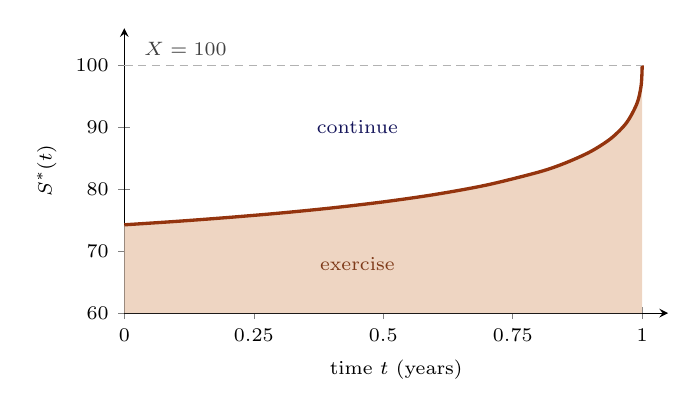
\begin{tikzpicture}[font=\footnotesize]
		\begin{axis}[
				width=0.7\textwidth, height=5.2cm,
				xmin=0, xmax=1.05, ymin=60, ymax=106,
				xtick={0,0.25,0.5,0.75,1}, ytick={60,70,80,90,100},
				xlabel={time $t$ (years)}, ylabel={$S^{*}(t)$},
				axis lines=left, axis line style={thin},
				label style={font=\scriptsize}, tick label style={font=\scriptsize},
				clip=false,
			]
			\addplot[draw=none, fill=RawSienna!15] coordinates {
					(0,60) (0.0,74.26) (0.1,74.81) (0.2,75.44) (0.3,76.15) (0.4,76.98) (0.5,77.96) (0.6,79.16) (0.7,80.69) (0.8,82.77) (0.85,84.19) (0.9,86.07) (0.94,88.23) (0.97,90.77) (0.99,93.88) (0.998,96.79) (1,100) (1,60)} \closedcycle;
			\addplot[RawSienna, very thick, smooth] coordinates {
					(0.0,74.26) (0.1,74.81) (0.2,75.44) (0.3,76.15) (0.4,76.98) (0.5,77.96) (0.6,79.16) (0.7,80.69) (0.8,82.77) (0.85,84.19) (0.9,86.07) (0.94,88.23) (0.97,90.77) (0.99,93.88) (0.998,96.79) (1,100)};
			\addplot[Gray!60, densely dashed] coordinates {(0,100) (1,100)};
			\node[font=\scriptsize, text=Gray!50!black, anchor=south west] at (axis cs:0.02,100) {$X=100$};
			\node[font=\scriptsize, text=RawSienna!80!black] at (axis cs:0.45,68) {exercise};
			\node[font=\scriptsize, text=MidnightBlue!80!black] at (axis cs:0.45,90) {continue};
		\end{axis}
	\end{tikzpicture}
	\caption{Exercise boundary of an American put with $X=100$, $r=8\%$,
		$\sigma=30\%$, expiring at $t=1$, computed by \autoref{alg:american-put}
		with 600 periods and bisection on $S$. Below the curve, immediate exercise
		is optimal. The boundary rises to $X$ at expiration.}
	\label{fig:exercise-boundary}
\end{figure}

\begin{intuition}
	Why does the put's boundary rise towards $X$?
	Waiting keeps the chance that the stock recovers, and that chance is worth less the less time remains; exercising early earns interest on $X$.
	As expiration approaches the first effect dies, so exercise becomes optimal at prices ever closer to the strike.
	For an American call the roles of the two effects are taken by dividends and interest on $X$, which reverses the direction.
\end{intuition}

%─────Chapter: Sensitivity Analysis──────────────────────────────────────────────────────────────────────────────────────────────────────────────────
\chapter{Sensitivity Analysis of Options}
\label{ch:greeks}

\source{Slides pp.~345--346}

\begin{flushright}
	\itshape Cleopatra's nose, had it been shorter,\\
	the whole face of the world\\
	would have been changed.\\
	\upshape --- Blaise Pascal (1623--1662)
\end{flushright}

\bigskip

\noindent Chapter~\ref{ch:pricing-models} produced a number.
This chapter asks how that number moves when each input moves --- which is what a trader holding the option actually needs to know, since it is the movements that have to be hedged.

%─────§ Greeks───────────────────────────────────────────────────────────────────────────────────────────────────────────────────────────────────────
\section{Sensitivity Measures (``The Greeks'')}
\label{sec:greeks}

\source{Slide p.~347}

How the value of a security changes relative to changes in a given parameter is key to hedging.
Duration (\autoref{sec:md-volatility}), for instance, is the bond's sensitivity to its yield.

\begin{remark}
	\vocab{希臘字母}（the Greeks）：選擇權價格對各個參數的偏導數——對股價是 Delta $\Delta$、對時間是 Theta $\Theta$、對股價的二階導數是 Gamma $\Gamma$、對波動率是 Vega $\Lambda$、對利率是 Rho $\rho$。它們之於選擇權，就像存續期間與凸性之於債券。
\end{remark}

\begin{notation}
	Throughout, $x$ is defined by \eqref{eq:bs-x},
	\[
		x \;=\; \frac{\ln(S/X)+\bigl(r+\sigma^{2}/2\bigr)\tau}{\sigma\sqrt{\tau}} ,
	\]
	and
	\[
		N'(y) \;=\; \frac{e^{-y^{2}/2}}{\sqrt{2\pi}} \;>\; 0
	\]
	is the density function of the standard normal distribution.
\end{notation}

Every closed-form Greek below follows from one identity, which is worth isolating.

\begin{lemma}
	\label{lem:bs-identity}
	\begin{equation}
		SN'(x) \;=\; Xe^{-r\tau}N'\bigl(x-\sigma\sqrt{\tau}\bigr) .
		\label{eq:bs-identity}
	\end{equation}
\end{lemma}

\begin{proof}
	$\dfrac{N'(x-\sigma\sqrt{\tau})}{N'(x)}=\exp\Bigl(x\sigma\sqrt{\tau}-\dfrac{\sigma^{2}\tau}{2}\Bigr)=\exp\Bigl(\ln\dfrac{S}{X}+r\tau\Bigr)=\dfrac{Se^{r\tau}}{X}$, using \eqref{eq:bs-x} for $x\sigma\sqrt{\tau}$.
\end{proof}

\begin{note}
	對 \eqref{eq:bs-call} 中任何出現在 $x$ 裡的參數 $\theta$ 微分時，chain rule 會產生
	\[
		SN'(x)\,\frac{\partial x}{\partial\theta}-Xe^{-r\tau}N'\bigl(x-\sigma\sqrt{\tau}\bigr)\,\frac{\partial\bigl(x-\sigma\sqrt{\tau}\bigr)}{\partial\theta} ,
	\]
	而由 \eqref{eq:bs-identity}，這會化簡成 $SN'(x)\,\partial(\sigma\sqrt{\tau})/\partial\theta$。
	所以只剩下對 $\theta$ 的\emph{顯式}依賴，以及 $\sigma\sqrt{\tau}$ 那一項。
\end{note}

%─────§ Delta───────────────────────────────────────────────────────────────────────────────────────────────────────────────────────────────────────
\section{Delta}
\label{sec:delta}

\source{Slide p.~348}

\begin{definition}
	\[
		\Delta \;\triangleq\; \frac{\partial f}{\partial S} ,
	\]
	where $f$ is the price of the derivative and $S$ is the price of the underlying asset.
\end{definition}

The delta of a portfolio of derivatives on the same underlying asset is the sum of their individual deltas, by elementary calculus.
The delta used in the BOPM, \eqref{eq:bopm-hb}, is the discrete analog.
The delta of a long stock is $1$.

\source{Slides pp.~349--350}

\begin{proposition}
	The delta of a European call on a non-dividend-paying stock equals
	\begin{equation}
		\frac{\partial C}{\partial S} \;=\; N(x) \;>\; 0 .
		\label{eq:delta-call}
	\end{equation}
	The delta of a European put equals
	\begin{equation}
		\frac{\partial P}{\partial S} \;=\; N(x)-1 \;=\; -N(-x) \;<\; 0 .
		\label{eq:delta-put}
	\end{equation}
\end{proposition}

\begin{proof}
	By the note after \autoref{lem:bs-identity}, $\partial C/\partial S=N(x)+SN'(x)\cdot\partial(\sigma\sqrt{\tau})/\partial S=N(x)$.
	For the put, differentiate parity $P=C-S+Xe^{-r\tau}$.
\end{proof}

So the deltas of a call and an otherwise identical put cancel each other when $N(x)=1/2$, i.e., when $x=0$, i.e., when
\begin{equation}
	X \;=\; Se^{(r+\sigma^{2}/2)\,\tau} .
	\label{eq:straddle-zero-delta}
\end{equation}
The straddle (\autoref{sec:combinations}) $C+P$ then has zero delta!

\begin{figure}[H]
	\centering
	\begin{tikzpicture}[font=\footnotesize]
		\begin{groupplot}[
				group style={group size=2 by 1, horizontal sep=1.5cm},
				width=0.48\textwidth, height=4.6cm,
				title style={font=\small, text=Gray!40!black},
				tick label style={font=\scriptsize},
				label style={font=\scriptsize},
				axis line style={thin}, tick align=outside,
				ymin=0, ymax=1.02,
			]
			\nextgroupplot[title={Delta (call)}, xlabel={Stock price}, xmin=0, xmax=80]
			\addplot[MidnightBlue!80!black, very thick, domain=1:80, samples=120] {gdelta(x,201/365)};
			\nextgroupplot[title={Delta (call)}, xlabel={Time to expiration (days)}, xmin=0, xmax=365]
			\addplot[Gray!60!black, thick, densely dotted, domain=1:365, samples=90] {gdelta(60,x/365)};
			\addplot[MidnightBlue!80!black, very thick, domain=1:365, samples=90] {gdelta(50,x/365)};
			\addplot[RawSienna, thick, dashed, domain=1:365, samples=90] {gdelta(40,x/365)};
		\end{groupplot}
	\end{tikzpicture}
	\caption{Call delta with $X=50$, $\sigma=30\%$, $r=8\%$; left with
		$\tau=201$ days, right against $\tau$ for $S=60$ (dotted, in the money),
		$S=50$ (solid, at the money) and $S=40$ (dashed, out of the money). The put
		delta is the same picture shifted down by $1$, by \eqref{eq:delta-put}.}
	\label{fig:delta}
\end{figure}

\begin{intuition}
	$N(x)$ is the hedge ratio of \autoref{sec:bopm-one-period} in the limit, and it reads like a probability of exercise.
	Deep in the money the call is the stock minus a bond, so $\Delta\to1$; deep out of the money it is nothing, so $\Delta\to0$.
	Near expiration there is no time left to change sides, so the curves on the right fan out to $1$, $1/2$ and $0$.
\end{intuition}

\subsection{Dividends, Straddles and Strangles}

\source{Slides pp.~351--353}

Suppose the stock pays a continuous dividend yield of $q$, and define $x$ by \eqref{eq:bs-x-q}.
Then
\[
	\frac{\partial C}{\partial S} \;=\; e^{-q\tau}N(x) \;>\; 0 ,
	\qquad
	\frac{\partial P}{\partial S} \;=\; -e^{-q\tau}N(-x) \;<\; 0 ,
\]
since \eqref{eq:bs-call-q} is \eqref{eq:bs-call} evaluated at $Se^{-q\tau}$.

Now consider an $X_{1}$-strike call and an $X_{2}$-strike put, $X_{1}\ge X_{2}$, otherwise identical.
Let
\begin{equation}
	x_{i} \;\triangleq\; \frac{\ln(S/X_{i})+\bigl(r-q+\sigma^{2}/2\bigr)\tau}{\sigma\sqrt{\tau}} .
	\label{eq:xi}
\end{equation}
Their deltas $e^{-q\tau}N(x_{1})$ and $-e^{-q\tau}N(-x_{2})$ sum to zero when $x_{1}=-x_{2}$, i.e., when $\ln(S/X_{1})+\ln(S/X_{2})=-(2r-2q+\sigma^{2})\tau$:
\begin{equation}
	\frac{S}{X_{1}} \;=\; \frac{X_{2}}{S}\,e^{-(2r-2q+\sigma^{2})\,\tau} .
	\label{eq:strangle-zero-delta}
\end{equation}
The strangle (\autoref{sec:combinations}) $C+P$ then has zero delta!
Demanding $X_{1}=X_{2}=X$ gives back a straddle, and \eqref{eq:strangle-zero-delta} becomes $X=Se^{(r-q+\sigma^{2}/2)\tau}$, generalizing \eqref{eq:straddle-zero-delta}.

\subsection{Delta Neutrality}

\source{Slide p.~354}

A position with a total delta equal to $0$ is \vocab{delta-neutral}.
A delta-neutral portfolio is immune to small price changes in the underlying asset, so creating one serves hedging purposes.
\begin{itemize}[nosep]
	\item A portfolio consisting of a call and $-\Delta$ shares of stock is delta-neutral.
	\item Short $\Delta$ shares of stock to hedge a long call; long $\Delta$ shares of stock to hedge a short call.
	\item In general, hedge a position in a security with delta $\Delta_{1}$ by shorting $\Delta_{1}/\Delta_{2}$ units of a security with delta $\Delta_{2}$.
\end{itemize}

\begin{remark}
	\vocab{Delta 中立}（delta-neutral）：整個部位的 delta 加總為 $0$，股價小幅變動時價值幾乎不變。避險比例 $\Delta_{1}/\Delta_{2}$ 的道理和 \autoref{sec:md-volatility} 之後的金額存續期間避險相同：要抵銷的是「金額」的變動。
\end{remark}

\begin{note}
	關鍵在「small」：delta neutrality 是一階的敘述，只在瞬間成立。
	$S$ 變動時 delta 也會跟著變 --- 變化率就是 gamma（\autoref{sec:gamma}）--- 所以 hedge 必須 rebalance，這就是 \autoref{sec:bopm-arbitrage-walk} 的連續時間版本。
\end{note}

%─────§ Theta───────────────────────────────────────────────────────────────────────────────────────────────────────────────────────────────────────
\section{Theta (Time Decay)}
\label{sec:theta}

\source{Slide p.~355}

\begin{definition}
	\vocab{Theta} is the rate of change of a security's value with respect to time,
	\[
		\Theta \;\triangleq\; -\frac{\partial f}{\partial\tau} \;=\; \frac{\partial f}{\partial t} .
	\]
\end{definition}

The minus sign is because $\tau$ is time \emph{to expiration}: as calendar time $t$ passes, $\tau$ shrinks.

\begin{proposition}
	For a European call on a non-dividend-paying stock,
	\[
		\Theta \;=\; -\frac{SN'(x)\,\sigma}{2\sqrt{\tau}}-rXe^{-r\tau}N\bigl(x-\sigma\sqrt{\tau}\bigr) \;<\; 0 ,
	\]
	and for a European put,
	\[
		\Theta \;=\; -\frac{SN'(x)\,\sigma}{2\sqrt{\tau}}+rXe^{-r\tau}N\bigl(-x+\sigma\sqrt{\tau}\bigr) .
	\]
\end{proposition}

\begin{proof}
	By the note after \autoref{lem:bs-identity}, $\partial C/\partial\tau$ is the explicit derivative of $-Xe^{-r\tau}$, namely $rXe^{-r\tau}N(x-\sigma\sqrt{\tau})$, plus $SN'(x)\,\partial(\sigma\sqrt{\tau})/\partial\tau=SN'(x)\,\sigma/(2\sqrt{\tau})$.
	For the put, differentiate parity: $\partial P/\partial\tau=\partial C/\partial\tau-rXe^{-r\tau}$, and $N(x-\sigma\sqrt{\tau})-1=-N(-x+\sigma\sqrt{\tau})$.
\end{proof}

The call loses value with the passage of time.
The put's theta can be negative or positive: deep in the money the second term wins, which is the European put worth less than its intrinsic value in \autoref{fig:option-value} --- waiting only delays receipt of $X$.

\source{Slides pp.~356--357}

\begin{figure}[H]
	\centering
	\begin{tikzpicture}[font=\footnotesize]
		\begin{groupplot}[
				group style={group size=2 by 1, horizontal sep=1.5cm},
				width=0.48\textwidth, height=4.6cm,
				title style={font=\small, text=Gray!40!black},
				tick label style={font=\scriptsize},
				label style={font=\scriptsize},
				axis line style={thin}, tick align=outside,
				xlabel={Stock price}, xmin=0, xmax=80,
			]
			\nextgroupplot[title={Theta (call)}, ymin=-6.5, ymax=0.2]
			\addplot[MidnightBlue!80!black, very thick, domain=1:80, samples=120] {gthetac(x,201/365)};
			\nextgroupplot[title={Theta (put)}, ymin=-2.5, ymax=4.2]
			\addplot[Gray!60, densely dashed] coordinates {(0,0) (80,0)};
			\addplot[RawSienna, very thick, domain=1:80, samples=120] {gthetap(x,201/365)};
		\end{groupplot}
	\end{tikzpicture}
	\caption{Theta (per year) with $X=50$, $\sigma=30\%$, $r=8\%$, $\tau=201$
		days. The call's is always negative and most negative near the money; the
		put's turns positive deep in the money, where it tends to $rXe^{-r\tau}$.}
	\label{fig:theta}
\end{figure}

Suppose the stock pays a continuous dividend yield of $q$, with $x$ as in \eqref{eq:bs-x-q}.
Then each formula gains an extra term:
\begin{align*}
	\Theta_{\text{call}} & \;=\; -\frac{SN'(x)\,\sigma\,e^{-q\tau}}{2\sqrt{\tau}}-rXe^{-r\tau}N\bigl(x-\sigma\sqrt{\tau}\bigr)+qSe^{-q\tau}N(x) , \\
	\Theta_{\text{put}}  & \;=\; -\frac{SN'(x)\,\sigma\,e^{-q\tau}}{2\sqrt{\tau}}+rXe^{-r\tau}N\bigl(-x+\sigma\sqrt{\tau}\bigr)-qSe^{-q\tau}N(-x) .
\end{align*}
The extra term is the derivative of $Se^{-q\tau}$ with respect to $-\tau$: a dividend-paying call gains from the passage of time insofar as fewer dividends remain to be paid out.\footnote{The slides write the first term without $e^{-q\tau}$; with $x$ from \eqref{eq:bs-x-q} the identity \eqref{eq:bs-identity} becomes $Se^{-q\tau}N'(x)=Xe^{-r\tau}N'(x-\sigma\sqrt{\tau})$, and the factor $e^{-q\tau}$ belongs there. Cf.\ the vega with dividends in \autoref{sec:vega}.}

%─────§ Gamma───────────────────────────────────────────────────────────────────────────────────────────────────────────────────────────────────────
\section{Gamma}
\label{sec:gamma}

\source{Slide p.~358}

\begin{definition}
	\vocab{Gamma} is the rate of change of the delta with respect to the price of the underlying asset,
	\[
		\Gamma \;\triangleq\; \frac{\partial^{2}f}{\partial S^{2}} .
	\]
\end{definition}

It measures how sensitive delta is to changes in the price of the underlying asset.
In practice, a portfolio with a high gamma needs be rebalanced more often to maintain delta neutrality.
Roughly, delta $\sim$ duration and gamma $\sim$ convexity (\autoref{sec:convexity}).

\begin{proposition}
	The gamma of a European call or put on a non-dividend-paying stock is
	\[
		\Gamma \;=\; \frac{N'(x)}{S\sigma\sqrt{\tau}} \;>\; 0 .
	\]
\end{proposition}

\begin{proof}
	Differentiate \eqref{eq:delta-call}: $\partial N(x)/\partial S=N'(x)\cdot\partial x/\partial S=N'(x)/(S\sigma\sqrt{\tau})$.
	The put's delta differs by the constant $-1$, so its gamma is the same.
\end{proof}

\begin{remark}
	Gamma 恆正，表示歐式選擇權的價值是 $S$ 的凸函數（與 \autoref{fig:option-value} 一致）。持有 gamma 為正的部位並做 delta 避險，股價大漲大跌都會賺一點（凸性），代價則是 theta 每天流失的時間價值。
\end{remark}

\source{Slides pp.~359--360}

\begin{figure}[H]
	\centering
	\begin{tikzpicture}[font=\footnotesize]
		\begin{groupplot}[
				group style={group size=2 by 1, horizontal sep=1.5cm},
				width=0.48\textwidth, height=4.6cm,
				title style={font=\small, text=Gray!40!black},
				tick label style={font=\scriptsize},
				label style={font=\scriptsize},
				yticklabel style={/pgf/number format/fixed, /pgf/number format/precision=2},
				axis line style={thin}, tick align=outside,
				ymin=0,
			]
			\nextgroupplot[title={Gamma (call/put)}, xlabel={Stock price}, xmin=0, xmax=80, ymax=0.042]
			\addplot[MidnightBlue!80!black, very thick, domain=1:80, samples=120] {ggamma(x,201/365)};
			\nextgroupplot[title={Gamma (call/put)}, xlabel={Time to expiration (days)}, xmin=0, xmax=365, ymax=0.4]
			\addplot[Gray!60!black, thick, densely dotted, domain=2:365, samples=120] {ggamma(60,x/365)};
			\addplot[MidnightBlue!80!black, very thick, domain=2:365, samples=120] {ggamma(50,x/365)};
			\addplot[RawSienna, thick, dashed, domain=2:365, samples=120] {ggamma(40,x/365)};
		\end{groupplot}
	\end{tikzpicture}
	\caption{Gamma with $X=50$, $\sigma=30\%$, $r=8\%$; right: $S=60$
		(dotted), $50$ (solid), $40$ (dashed). The at-the-money gamma grows like
		$1/\sqrt{\tau}$ as $\tau\to0$; the others die out.}
	\label{fig:gamma}
\end{figure}

Gamma is maximized when the option is nearly at the money, namely at
\[
	S \;=\; Xe^{-(r+3\sigma^{2}/2)\,\tau} .
\]
Indeed $\partial\ln\Gamma/\partial S=-x/(S\sigma\sqrt{\tau})-1/S$, which vanishes at $x=-\sigma\sqrt{\tau}$; substituting into \eqref{eq:bs-x} gives the formula.
As the at-the-money option approaches expiration, its gamma tends to rise, like $1/\sqrt{\tau}$; the gammas of other options, however, tend to zero, because $N'(x)\to0$ faster as $\abs{x}\to\infty$.

\begin{intuition}
	Near expiration an at-the-money option's delta is about to jump from $0$ to $1$ across the strike (the right panel of \autoref{fig:delta}); a jump is an infinite slope, so the delta's slope --- gamma --- explodes there.
	This is the hedger's nightmare: at-the-money options close to expiry need constant rebalancing.
\end{intuition}

%─────§ Vega────────────────────────────────────────────────────────────────────────────────────────────────────────────────────────────────────────
\section{Vega}
\label{sec:vega}

\source{Slide p.~361}

\begin{definition}
	\vocab{Vega} (also lambda, kappa, sigma, zeta) is the rate of change of a security's value with respect to the volatility of the underlying asset,
	\[
		\Lambda \;\triangleq\; \frac{\partial f}{\partial\sigma} .
	\]
\end{definition}

Vega is not Greek.
Alexander (2001): ``This is a term that was invented by Americans, and intended to sound like a Greek letter.''

Volatility often changes over time (\autoref{sec:time-dependent}), and a security with a high vega is very sensitive to changes in, or estimation error of, the volatility.

\begin{proposition}
	The vega of a European call or put on a non-dividend-paying stock is
	\[
		\Lambda \;=\; S\sqrt{\tau}\,N'(x) \;>\; 0 .
	\]
\end{proposition}

\begin{proof}
	$\sigma$ enters \eqref{eq:bs-call} only through $x$, so by the note after \autoref{lem:bs-identity},
	\[
		\frac{\partial C}{\partial\sigma} \;=\; SN'(x)\,\frac{\partial(\sigma\sqrt{\tau})}{\partial\sigma} \;=\; S\sqrt{\tau}\,N'(x) .
	\]
	By parity the put's vega is the same.
\end{proof}

So higher volatility raises the option value, which incidentally guarantees the uniqueness of the implied volatility in \autoref{sec:implied-vol}.

\source{Slides pp.~362--364}

\begin{figure}[H]
	\centering
	\begin{tikzpicture}[font=\footnotesize]
		\begin{groupplot}[
				group style={group size=2 by 1, horizontal sep=1.5cm},
				width=0.48\textwidth, height=4.6cm,
				title style={font=\small, text=Gray!40!black},
				tick label style={font=\scriptsize},
				label style={font=\scriptsize},
				axis line style={thin}, tick align=outside,
				ymin=0,
			]
			\nextgroupplot[title={Vega (call/put)}, xlabel={Stock price}, xmin=0, xmax=80, ymax=15]
			\addplot[MidnightBlue!80!black, very thick, domain=1:80, samples=120] {gvega(x,201/365)};
			\nextgroupplot[title={Vega (call/put)}, xlabel={Time to expiration (days)}, xmin=0, xmax=365, ymax=19]
			\addplot[Gray!60!black, thick, densely dotted, domain=1:365, samples=90] {gvega(60,x/365)};
			\addplot[MidnightBlue!80!black, very thick, domain=1:365, samples=90] {gvega(50,x/365)};
			\addplot[RawSienna, thick, dashed, domain=1:365, samples=90] {gvega(40,x/365)};
		\end{groupplot}
	\end{tikzpicture}
	\caption{Vega with $X=50$, $\sigma=30\%$, $r=8\%$; right: $S=60$
		(dotted), $50$ (solid), $40$ (dashed). Every curve vanishes as
		$\tau\to0$.}
	\label{fig:vega}
\end{figure}

Note that\footnote{Reiss \& Wystup (2001).}
\begin{equation}
	\Lambda \;=\; \tau\sigma S^{2}\,\Gamma ,
	\label{eq:vega-gamma}
\end{equation}
as the two formulas show at a glance.
If the stock pays a continuous dividend yield of $q$, then
\[
	\Lambda \;=\; Se^{-q\tau}\sqrt{\tau}\,N'(x) ,
\]
where $x$ is defined in \eqref{eq:bs-x-q}.

Vega is maximized when $x=0$, i.e., when $S=Xe^{-(r-q+\sigma^{2}/2)\,\tau}$, and declines very fast as $S$ moves away from that peak.

\begin{note}
	「Maximized」需要加個條件。
	固定 $S$ 時，$x=0$ 使 $N'(x)$ 最大，因此也使 vega 在\emph{不同 strike} $X$ 之間最大。
	若固定 strike、把 vega 看成 $S$ 的函數，多出來的因子 $S$ 會讓峰值移動：$\partial\ln\Lambda/\partial S=(1-x/(\sigma\sqrt{\tau}))/S$ 在 $x=\sigma\sqrt{\tau}$ 時為零，也就是 $S=Xe^{-(r-q-\sigma^{2}/2)\tau}$ --- 這正是 \autoref{fig:vega} 左圖的峰值位置。
\end{note}

Now consider a portfolio consisting of an $X_{1}$-strike call $C$ and a \emph{short} $X_{2}$-strike put $P$, $X_{1}\ge X_{2}$.
Their vegas are $Se^{-q\tau}\sqrt{\tau}N'(x_{i})$ with $x_{i}$ as in \eqref{eq:xi}, and they cancel out when $x_{1}=-x_{2}$, since $N'$ is even.
This leads to \eqref{eq:strangle-zero-delta} --- the same condition that gave zero delta for the strangle $C+P$.

\source{Slides p.~365}

Note that $\tau\to0$ implies $\Lambda\to0$, which answers the question in \autoref{sec:implied-vol}.
The Black--Scholes formula also implies
\[
	C\to S , \qquad P\to Xe^{-r\tau} , \qquad\text{as }\sigma\to\infty ,
\]
since $x\to\infty$ and $x-\sigma\sqrt{\tau}\to-\infty$.
These are the \emph{upper} ends of the ranges allowed by no-arbitrage --- recall $C\ge\max(S-Xe^{-r\tau},0)$ (the proof of \autoref{thm:merton-no-early}) and $P\ge\max(Xe^{-r\tau}-S,0)$ (\autoref{lem:put-bound}), the lower ends, which are the limits as $\sigma\to0$.
These boundary conditions are handy for some numerical methods.

%─────§ Rho─────────────────────────────────────────────────────────────────────────────────────────────────────────────────────────────────────────
\section{Rho}
\label{sec:rho}

\source{Slides pp.~366--367}

\begin{definition}
	\vocab{Rho} is the rate of change in a security's value with respect to interest rates,
	\[
		\rho \;\triangleq\; \frac{\partial f}{\partial r} .
	\]
\end{definition}

\begin{proposition}
	The rho of a European call and of a European put on a non-dividend-paying stock are, respectively,
	\[
		X\tau e^{-r\tau}N\bigl(x-\sigma\sqrt{\tau}\bigr) \;>\; 0 ,
		\qquad
		-X\tau e^{-r\tau}N\bigl(-x+\sigma\sqrt{\tau}\bigr) \;<\; 0 .
	\]
\end{proposition}

\begin{proof}
	$r$ does not enter $\sigma\sqrt{\tau}$, so only the explicit $e^{-r\tau}$ contributes: $\partial C/\partial r=X\tau e^{-r\tau}N(x-\sigma\sqrt{\tau})$.
	Parity gives the put's: $\partial P/\partial r=\partial C/\partial r-X\tau e^{-r\tau}$.
\end{proof}

A call holder will pay $X$ later, a put holder will receive it later; raising $r$ shrinks $\mathrm{PV}(X)$, which helps the first and hurts the second.

\begin{figure}[H]
	\centering
	\begin{tikzpicture}[font=\footnotesize]
		\begin{groupplot}[
				group style={group size=2 by 1, horizontal sep=1.5cm},
				width=0.48\textwidth, height=4.6cm,
				title style={font=\small, text=Gray!40!black},
				tick label style={font=\scriptsize},
				label style={font=\scriptsize},
				axis line style={thin}, tick align=outside,
				xlabel={Stock price}, xmin=0, xmax=80,
			]
			\nextgroupplot[title={Rho (call)}, ymin=0, ymax=28]
			\addplot[MidnightBlue!80!black, very thick, domain=1:80, samples=120] {grhoc(x,201/365)};
			\nextgroupplot[title={Rho (put)}, ymin=-28, ymax=0]
			\addplot[RawSienna, very thick, domain=1:80, samples=120] {grhop(x,201/365)};
		\end{groupplot}
	\end{tikzpicture}
	\caption{Rho with $X=50$, $\sigma=30\%$, $r=8\%$, $\tau=201$ days. Deep in
		the money the call's rho tends to $X\tau e^{-r\tau}\approx26$, the rate
		sensitivity of the bond $Xe^{-r\tau}$ it effectively shorts.}
	\label{fig:rho}
\end{figure}

%─────§ Numerical Greeks────────────────────────────────────────────────────────────────────────────────────────────────────────────────────────────
\section{Numerical Greeks}
\label{sec:numerical-greeks}

\source{Slide p.~368}

Closed forms exist only for the simplest options; for an American put, say, the Greeks must be computed numerically.
Take delta as an example.
A standard method computes the finite difference
\[
	\frac{f(S+\Delta S)-f(S-\Delta S)}{2\Delta S} ,
\]
which roughly doubles the computation time of evaluating the derivative itself (two extra pricings).

\subsection{An Alternative Numerical Delta}

\source{Slide p.~369}

Use intermediate results of the binomial tree algorithm instead.\footnote{Pelsser \& Vorst (1994).}
When the algorithm reaches the end of the first period, $f_{u}$ and $f_{d}$ are computed; they are the derivative values at stock prices $Su$ and $Sd$.
Delta is approximated by
\begin{equation}
	\frac{f_{u}-f_{d}}{Su-Sd} ,
	\label{eq:num-delta}
\end{equation}
at essentially zero extra cost --- stop \autoref{alg:american-put} one step early and return $\bigl(P[0]-P[1]\bigr)/(Su-Sd)$.
This is just \eqref{eq:bopm-hb}.

\subsection{Extended Binomial Tree}

\source{Slide p.~370}

Strictly speaking, \eqref{eq:num-delta} is the delta at time $\Delta t$, not now.
An improved method starts the tree two periods \emph{before} now (\autoref{fig:extended-tree}), so that the present time is the third column, with nodes $Su/d$, $S$, $Sd/u$.
Delta is then
\[
	\frac{f_{u/d}-f_{d/u}}{Su/d-Sd/u} ,
\]
and gamma is
\[
	\frac{\dfrac{f_{u/d}-f}{Su/d-S}-\dfrac{f-f_{d/u}}{S-Sd/u}}{(Su/d-Sd/u)/2} ,
\]
both at the present time.

\begin{figure}[H]
	\centering
	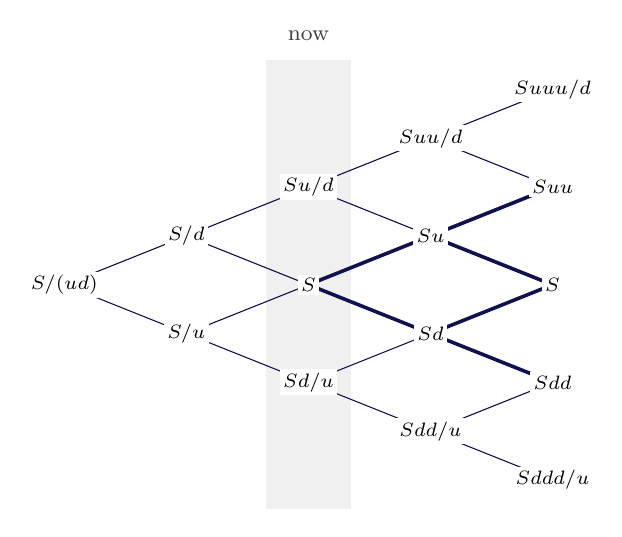
\begin{tikzpicture}[font=\scriptsize, x=1.55cm, y=0.62cm,
			ln/.style={MidnightBlue!70!black}, every node/.style={inner sep=1.2pt}]
		\fill[Gray!12] (1.65,-4.6) rectangle (2.35,4.6);
		\node[font=\footnotesize, text=Gray!50!black] at (2,5.1) {now};
		\foreach \t in {0,...,4}{
				\foreach \i in {0,...,\t}{
						\pgfmathtruncatemacro{\k}{\t-2*\i}
						\ifnum\t<4
							\pgfmathtruncatemacro{\kk}{\k+1}
							\pgfmathtruncatemacro{\km}{\k-1}
							\pgfmathtruncatemacro{\tn}{\t+1}
							\draw[ln, thin] (\t,\k) -- (\tn,\kk);
							\draw[ln, thin] (\t,\k) -- (\tn,\km);
						\fi
					}
			}
		\draw[ln, line width=1.3pt] (3,1) -- (2,0) -- (3,-1);
		\draw[ln, line width=1.3pt] (4,2) -- (3,1) -- (4,0) -- (3,-1) -- (4,-2);
		\node[fill=white] at (0,0) {$S/(ud)$};
		\node[fill=white] at (1,1) {$S/d$};
		\node[fill=white] at (1,-1) {$S/u$};
		\node[fill=white] at (2,2) {$Su/d$};
		\node[fill=white] at (2,0) {$S$};
		\node[fill=white] at (2,-2) {$Sd/u$};
		\node[fill=white] at (3,3) {$Suu/d$};
		\node[fill=white] at (3,1) {$Su$};
		\node[fill=white] at (3,-1) {$Sd$};
		\node[fill=white] at (3,-3) {$Sdd/u$};
		\node[fill=white] at (4,4) {$Suuu/d$};
		\node[fill=white] at (4,2) {$Suu$};
		\node[fill=white] at (4,0) {$S$};
		\node[fill=white] at (4,-2) {$Sdd$};
		\node[fill=white] at (4,-4) {$Sddd/u$};
	\end{tikzpicture}
	\caption{The extended binomial tree: the original tree (bold) with time
		extended two periods before the present. With $ud=1$, $S/(ud)=S$, and the
		present column holds $Su^{2}$, $S$, $Sd^{2}$.}
	\label{fig:extended-tree}
\end{figure}

\subsection{Numerical Gamma}

\source{Slide p.~371}

On the ordinary tree, gamma is read off the second period.
At the stock price $(Suu+Sud)/2$, delta is approximately $(f_{uu}-f_{ud})/(Suu-Sud)$; at $(Sud+Sdd)/2$, it is approximately $(f_{ud}-f_{dd})/(Sud-Sdd)$.
Gamma is the rate of change in deltas between these two prices:
\begin{equation}
	\frac{\dfrac{f_{uu}-f_{ud}}{Suu-Sud}-\dfrac{f_{ud}-f_{dd}}{Sud-Sdd}}{(Suu-Sdd)/2} .
	\label{eq:num-gamma}
\end{equation}

\subsection{Alternative Numerical Delta and Gamma}

\source{Slide p.~372}

Let $\epsilon\triangleq\ln u$ and think in terms of $\ln S$, where the CRR lattice is evenly spaced.
Since $\partial f/\partial S=\frac1S\,\partial f/\partial\ln S$ and $\partial^{2}f/\partial S^{2}=\frac{1}{S^{2}}\bigl(\partial^{2}f/\partial(\ln S)^{2}-\partial f/\partial\ln S\bigr)$,
\[
	\left(\frac{f_{u}-f_{d}}{2\epsilon}\right)\frac{1}{S}
\]
approximates the numerical delta, and
\[
	\left(\frac{f_{uu}-2f_{ud}+f_{dd}}{\epsilon^{2}}-\frac{f_{uu}-f_{dd}}{2\epsilon}\right)\frac{1}{S^{2}}
\]
approximates the numerical gamma.\footnote{See p.~692 of the slides, where the grid has spacing $\epsilon$ in $\ln S$. On the binomial tree, $f_{uu},f_{ud},f_{dd}$ are $2\epsilon$ apart, so $\epsilon$ in the gamma formula should then read $2\epsilon$.}

\subsection{Finite Difference Fails for Numerical Gamma}
\label{sec:numerical-gamma-fails}

\source{Slide p.~373}

Numerical differentiation gives
\[
	\frac{f(S+\Delta S)-2f(S)+f(S-\Delta S)}{(\Delta S)^{2}} .
\]
It does not work, and in general calculating gamma is a hard problem numerically --- recall the floating-point disaster of \autoref{fig:fp-error}.
But here the failure is structural, not only floating-point.

\begin{figure}[H]
	\centering
	\begin{tikzpicture}[font=\footnotesize]
		\begin{groupplot}[
				group style={group size=2 by 1, horizontal sep=1.5cm},
				width=0.48\textwidth, height=4.6cm,
				title style={font=\small, text=Gray!40!black},
				tick label style={font=\scriptsize},
				label style={font=\scriptsize},
				axis line style={thin}, tick align=outside,
				xlabel={Stock price $S$}, xmin=0, xmax=450,
				clip=false,
			]
			\nextgroupplot[title={Tree value $f(S)$}, ymin=0, ymax=380]
			\addplot[MidnightBlue!80!black, very thick, domain=0:450, samples=181]
			{(0.343*max(0,3.375*x-150)+0.441*max(0,1.125*x-150)+0.189*max(0,0.375*x-150)+0.027*max(0,0.125*x-150))/1.728};
			\draw[Gray!60, densely dotted] (axis cs:44.44,0) -- (axis cs:44.44,380);
			\draw[Gray!60, densely dotted] (axis cs:133.33,0) -- (axis cs:133.33,380);
			\draw[Gray!60, densely dotted] (axis cs:400,0) -- (axis cs:400,380);
			\nextgroupplot[title={Finite-difference delta}, ymin=0, ymax=1.1]
			\addplot[RawSienna, very thick, const plot] coordinates {
					(0,0) (44.44,0.66992) (133.33,0.95703) (400,0.99805) (450,0.99805)};
		\end{groupplot}
	\end{tikzpicture}
	\caption{The three-period call of \autoref{eg:bopm-three-period} as a function
		of the initial price $S$ (with $u$, $d$, $R$, $X$ fixed). It is piecewise
		linear with kinks at $S=X/(u^{j}d^{3-j})$ (dotted), so a small-step
		finite-difference delta is a ladder, and the finite-difference gamma is $0$
		almost everywhere and huge at the kinks.}
	\label{fig:numerical-gamma-fails}
\end{figure}

\begin{note}
	原因來自 \eqref{eq:bopm-call-n}：固定 $u$、$d$、$\hat{r}$、$n$ 時，tree 算出的 option 價值是目前股價 $S$ 的連續 \emph{piecewise linear} 函數，kink（折點）在 $S=Xu^{-j}d^{-(n-j)}$，$j=0,1,\ldots,n$。\footnote{課本 Section 10.2.1。}
	\begin{itemize}[nosep]
		\item 若 $\Delta S$ 很小，且離 $S$ 不到 $\Delta S$ 的範圍內沒有 kink，則 $f'(S-\Delta S)=f'(S)=f'(S+\Delta S)$，數值 gamma 恰好為零。
		\item 若有 kink $\bar{S}$ 滿足 $S-\Delta S<\bar{S}<S$，令 $\delta>0$ 為該處斜率的跳躍量；則數值 gamma 等於 $\delta\,(\bar{S}-S+\Delta S)/(\Delta S)^{2}$，當 $\Delta S$ 變小時可能變得非常大。
	\end{itemize}
	常見的「把 step size 調小」並沒有幫助，反而會更糟。
\end{note}

But why did the binomial tree version \eqref{eq:num-gamma} work?
Because its step is not a free parameter: the nodes $Suu$, $Sud$, $Sdd$ are spaced by the factor $u/d$, which is exactly the spacing of the kinks.
Each of its two difference quotients spans one full linear piece of the tree's own value function, so the second difference sees every kink with the same weight instead of catching one by accident.\footnote{Exercise 10.2.1 of the textbook.}

\begin{moral}
	Differentiate a numerical method on its own grid.
	A finite difference with a step finer than the method's resolution measures the method's artefacts, not the derivative.
\end{moral}

\subsection{Other Numerical Greeks}

\source{Slide p.~374}

The theta can be computed on the tree as
\[
	\frac{f_{ud}-f}{2(\tau/n)} ,
\]
since $Sud=S$: the same stock price two periods later.
In fact, the theta of a European option can be derived from delta and gamma, by an equation we shall meet later in the course.
The vega of a European option can be derived from gamma, by \eqref{eq:vega-gamma}.
For rho, there seems no alternative but to run the binomial tree algorithm twice.
